%! Author = ASUS
%! Date = 3/27/2023

% Preamble
\documentclass[11pt]{article}

% Packages
\usepackage{amsmath}
\usepackage{lipsum}
\usepackage{wasysym}
\usepackage{subcaption}
\usepackage{adjustbox}
\usepackage{multirow}
\usepackage{graphicx}
\usepackage{float}
\usepackage{listings}
\usepackage{xcolor}
\usepackage{pgfplots}
\lstset{basicstyle=\ttfamily,
  showstringspaces=false,
  commentstyle=\color{red},
  keywordstyle=\color{blue}
}

\graphicspath{{./images}}

% Document
\begin{document}
    \section{Dataset}
    \paragraph{Aerial Point Cloud:} An extensive collection of 3D points is obtained from the city of Padova
    using an airplane. The covered region spans 1600m by 1000m, and the average nearest neighbor distance
    of points is 0.63m. The dataset contains a total of 3,583,803 points, figure \ref{fig:ply_aerial_all}.
    \paragraph{Ground Point Clouds:} 10 dense point clouds are created using the Structure from Motion techniques.
    These datasets are further refined using Pixel-Perfect algorithm. Each dataset comprises an average of
    60 frames extracted from a 30-second undistorted video. The video was recorded at a frame rate of 60 fps,
    resulting in the generation of point clouds at a rate of 2 pictures per second. The resolution of each image
    is 1920*1088 pixels, and the distance covered in each dataset ranges from 80 to 120 meters.

    \begin{figure}
    \centering
    \includegraphics[width=\textwidth,height=\textheight,keepaspectratio]{images/experiment/ply_aerial_all}
    \caption{The aerial point cloud}
    \label{fig:ply_aerial_all}
    \end{figure}

    \section{Point Cloud Registration}
    The objective is to align the ground point cloud with the aerial point cloud. Initially, we attempted
    to register the point cloud using traditional global and local algorithms like FPFH feature matching,
    RANSAC, and ICP. However, due to significant differences in the nature of the datasets, the results were
    too poor. The aerial point cloud primarily consists of street points and building roofs, as it is captured
    from above. While, the ground point cloud contains street points and building walls. Therefore, we need to
    find the common features and simplify the problem. The new pipeline could be described as follows:
    \begin{enumerate}
        \item It was observed that viewing both point clouds from above, aligned with the z-axis, provides
        valuable information. The first step is to align the point clouds with the z-axis. The aerial
        point cloud is already aligned. The ground point cloud is segmented into planes, and the plane
        with the highest point count is identified as the street plane, since it is the common plane among
        all streets and directions and so more points must be related to the ground plane. Then,
        the rotation matrix between the normal vector of the street plane and the (x=0, y=0, z=1) vector
        is computed and applied to the entire ground point cloud. This step roughly determines the rotation
        around x and y axes.

        \item From the top point of view, It is seen that the most discriminative feature among the datasets
        is the angles of streets and crossroads. So, the data of vertical walls in ground dataset and roofs
        in aerial dataset has no use. Therefore, both point clouds are sliced along the z-axis with a certain
        threshold, and the half related to the streets is remained. In figure \ref{fig:ply_sliced}, the similarity of
        both ground and aerial point clouds are visible.
        \begin{figure}
            \centering
            \begin{subfigure}{0.45\textwidth}
                \centering
                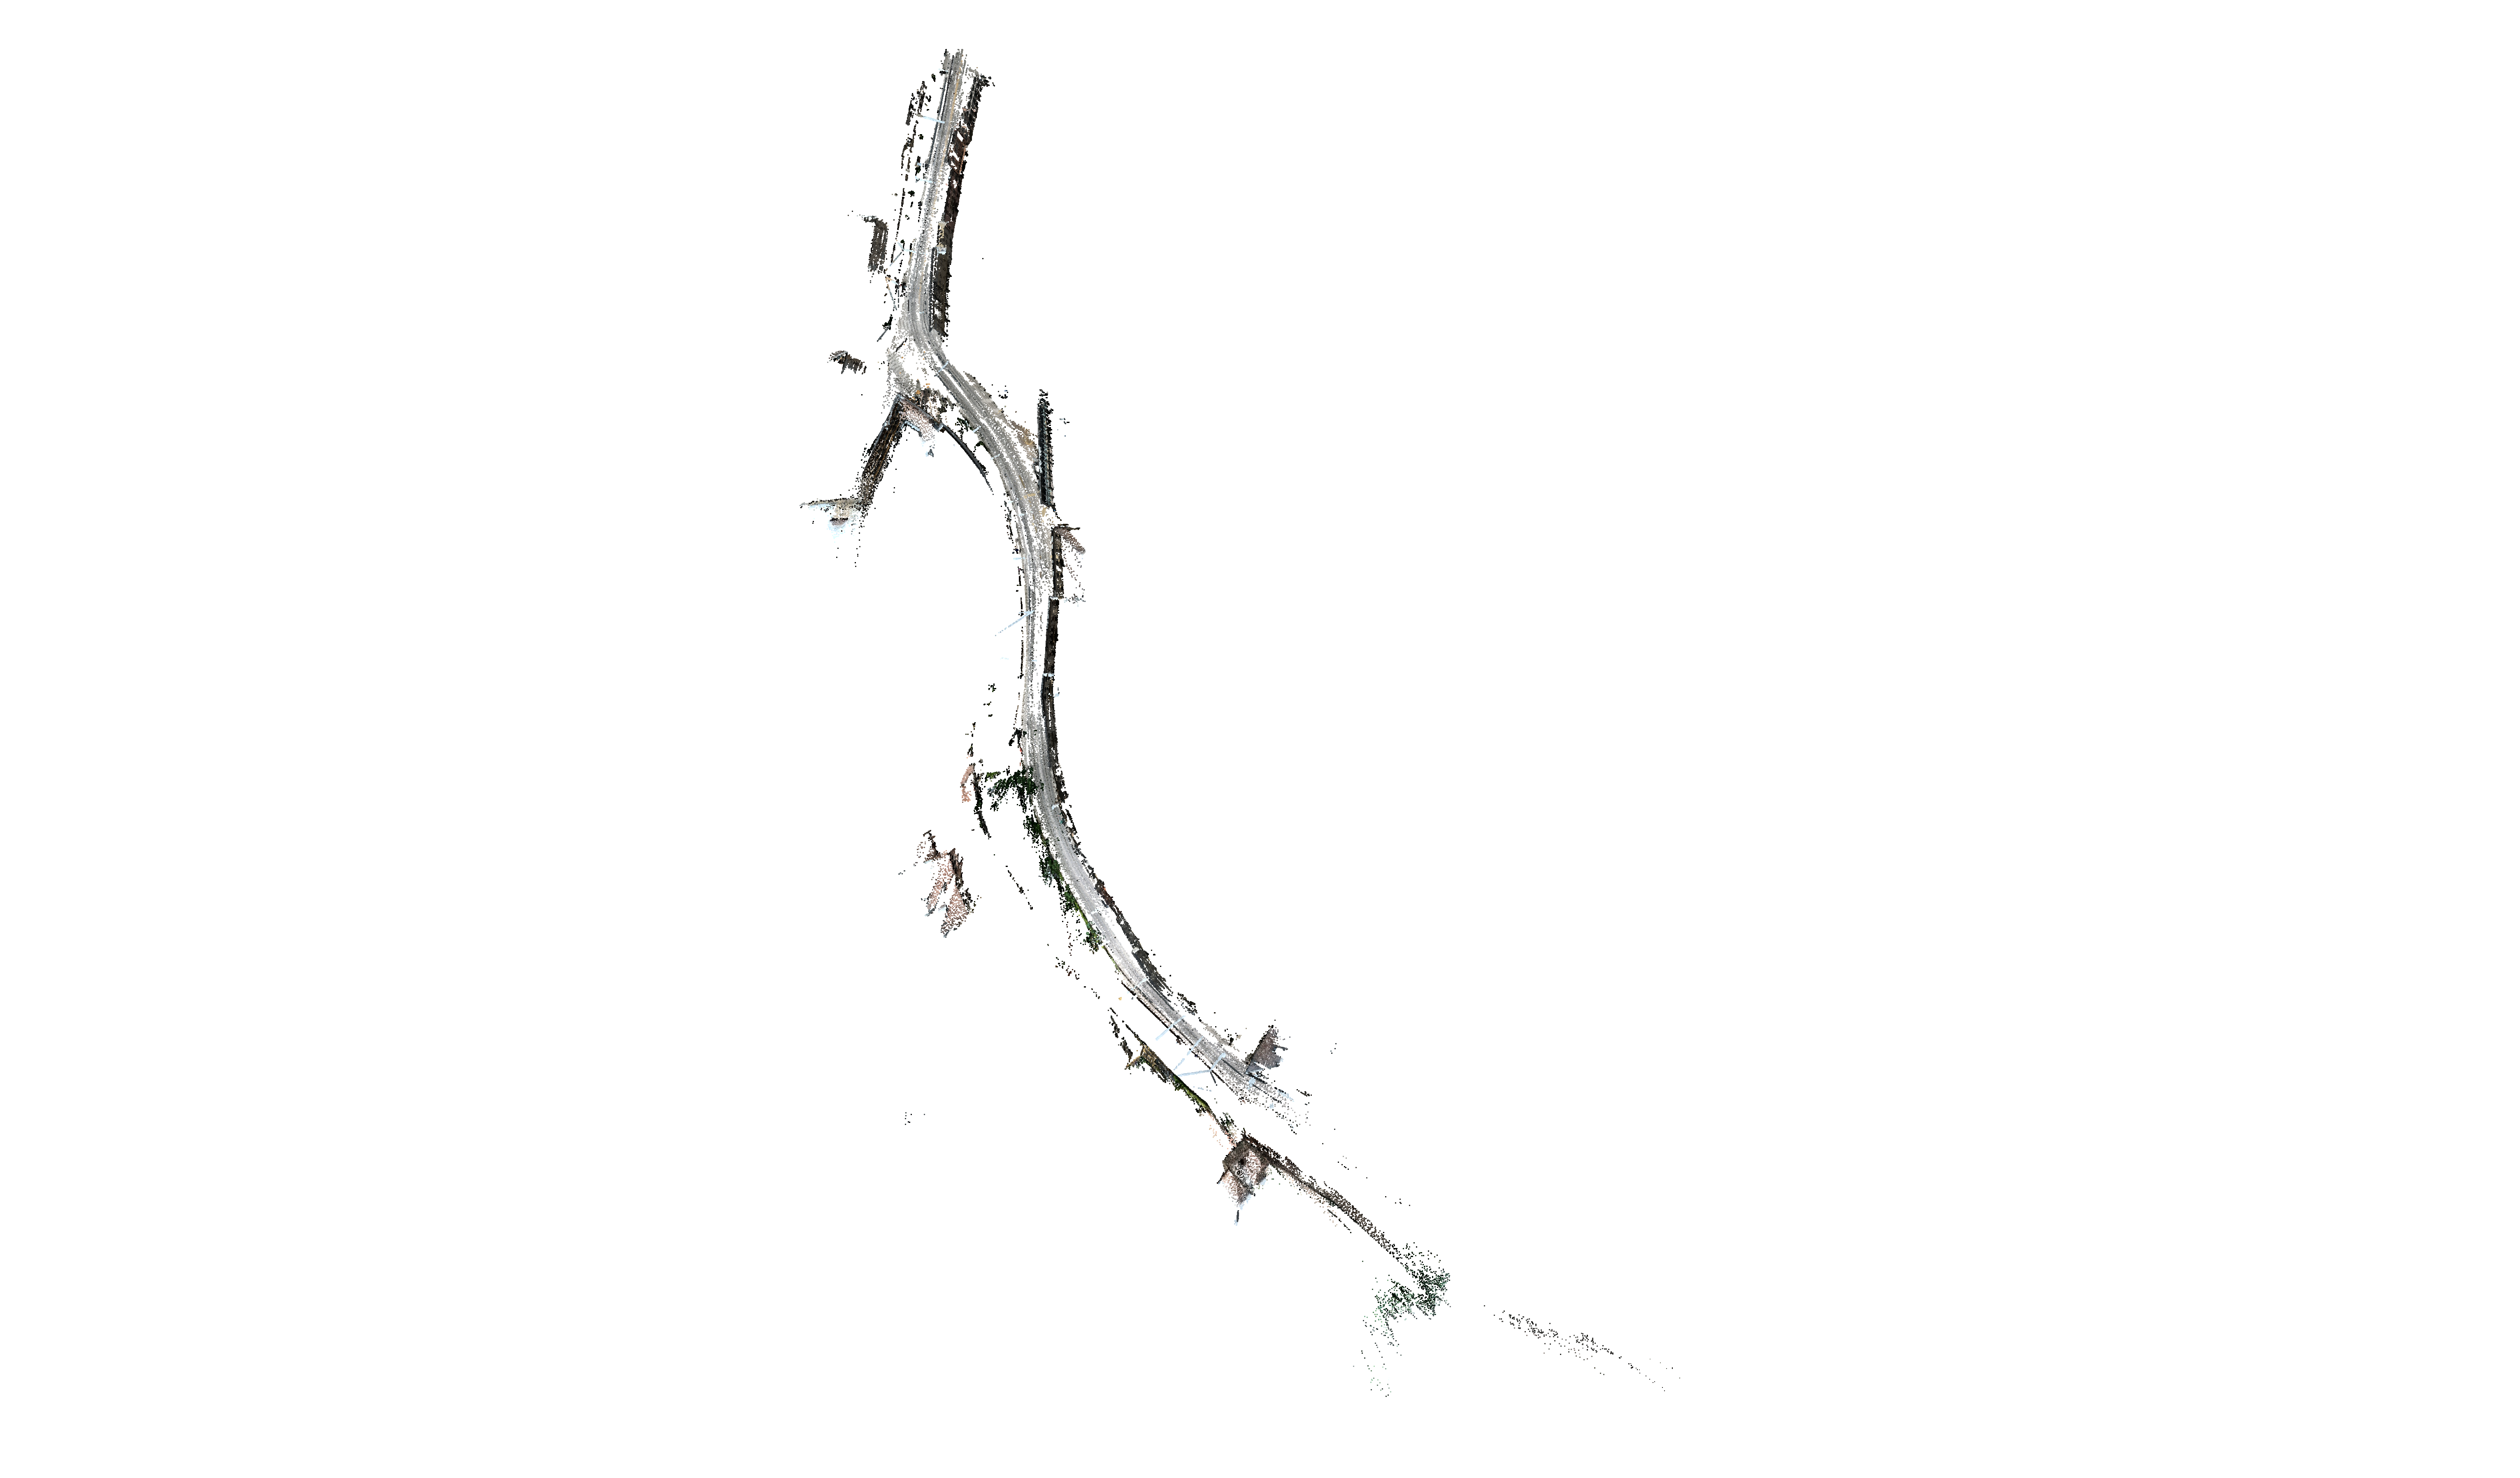
\includegraphics[width=\linewidth]{images/experiment/ply_sliced_ground}
                \caption{Ground Point Cloud}
            \end{subfigure}
            \hfill
            \begin{subfigure}{0.45\textwidth}
                \centering
                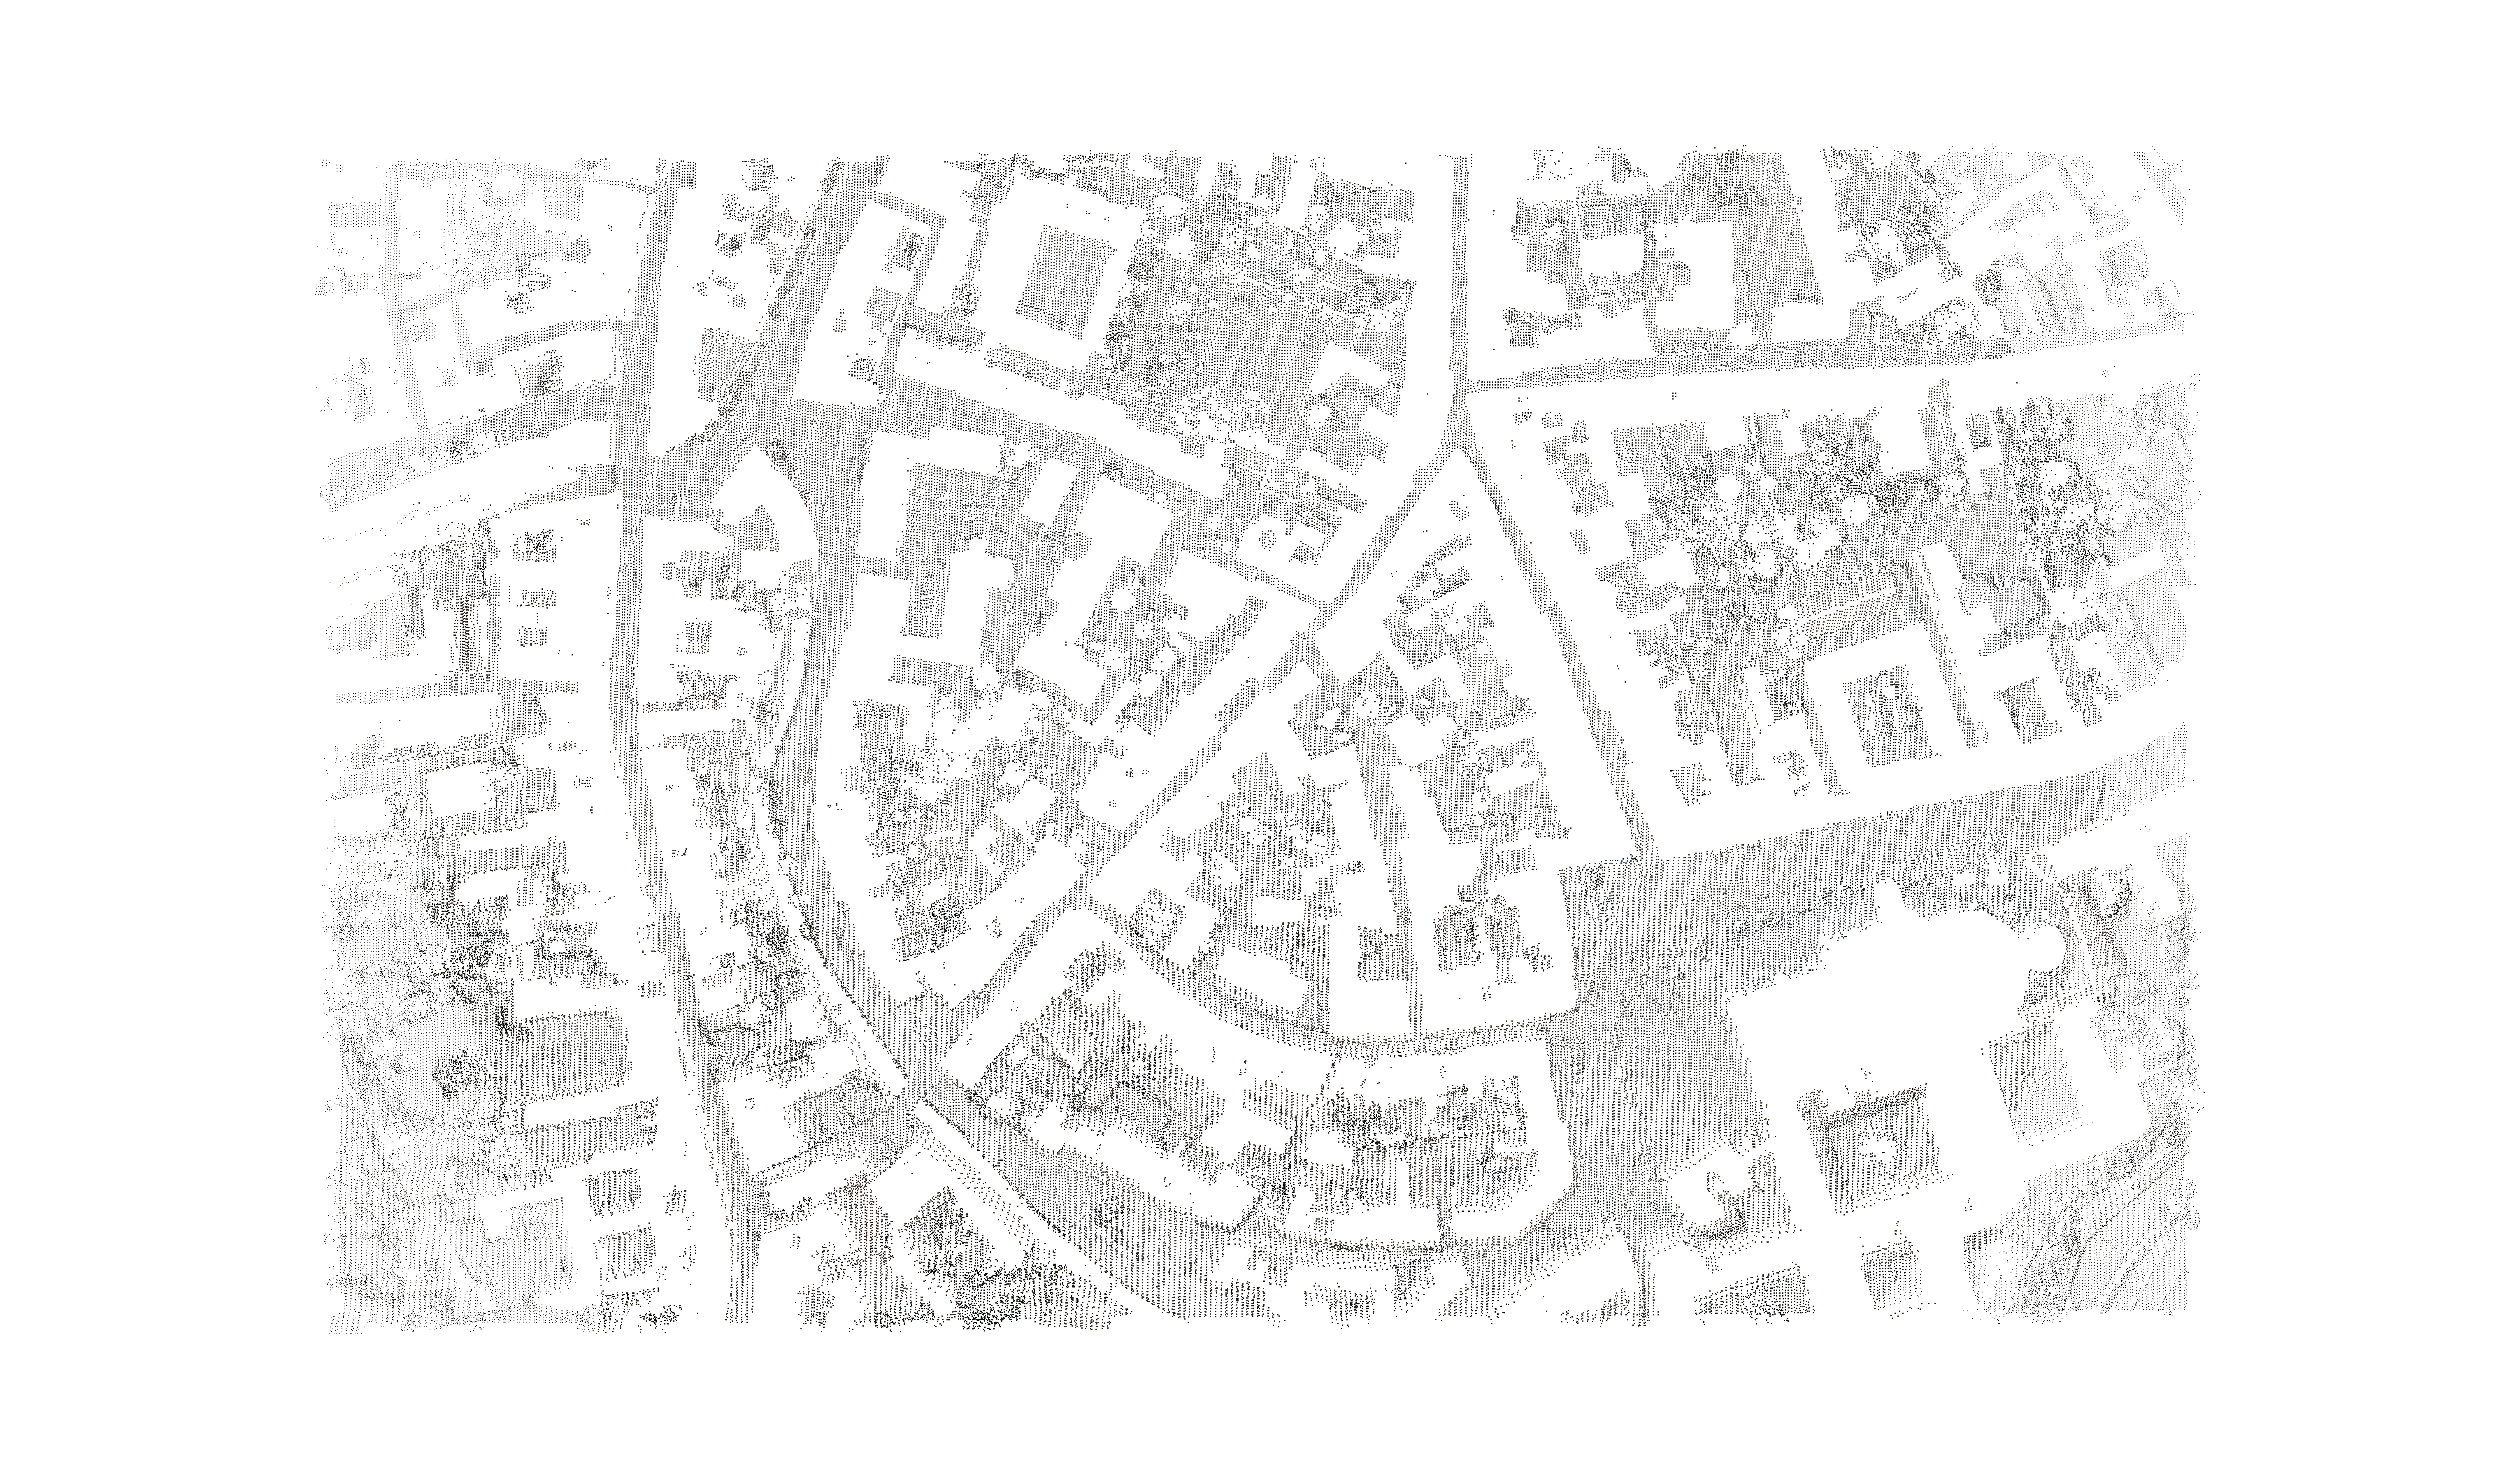
\includegraphics[width=\linewidth]{images/experiment/ply_sliced_aerial}
                \caption{Aerial Point Cloud}
            \end{subfigure}
            \caption{Point clouds sliced from the top viewpoint}
            \label{fig:ply_sliced}
        \end{figure}

        \item Since the generated point clouds has the up-to-scale problem, it is needed to normalize the
        coordinate values across all datasets. This step does not scale the ground point clouds to the actual size
        in aerial point cloud. However, it ensures that the average minimum distance between the points is 1px.
        Each point cloud is scaled by the factor of 1 divided by the average of the minimum distance to the nearest point.

        \item A 2D binary map is generated for each point cloud considering only x and y coordinates of each 3D point.
        The dimensions of the map are determined by calculating the difference between the maximum and minimum x and y
        coordinates of all points and dividing it by a predefined resolution value. Each cell in the map is assigned
        a value of 1 if at least one point's x and y coordinates fall within that cell, indicating the presence of
        points in that area. Conversely, if there are no points corresponding to the respective x and y coordinates,
        the cell is marked as 0. In the binary grid map for Ground Point Cloud, considering that each point cloud is
        generated from a sequence of video frames, the camera pose of the middle frame is regarded as the ground truth
        center position for the entire dataset. To evaluate the registration method's robustness and generalization,
        3 aerial point clouds are considered for each ground dataset. These aerial point clouds share the same center
        as the aforementioned ground point cloud, but they differ in distance from the center. They are categorized
        as "easy," "medium," and "hard" with distances of 100, 150, and 200 meters from each direction, respectively.
        The binary grid map is generated for these aerial point clouds using the same logic as the binary grid map
        created for the ground point clouds.

        \item To localize the ground grid map within the aerial grid maps, various methods were explored, including
        2D feature matching, crossroad detection based on point counting, and training convolutional neural networks,
        etc. Among these approaches, template matching has the best results. The template matching process involves
        comparing a small template image, which represents the desired pattern (in this case, the ground grid map),
        with different regions of the target image (the aerial grid map). The objective is to identify the best match
        or similarity between the template and the target image. This is achieved by moving a window across the target
        image and comparing the template with each window. We also extended the algorithm to also includes different
        scaling and rotation parameters. The template is rotated upto 360 degrees with an interval of 10 degrees and
        scaled from 10\% to 200\% of its initial size, increasing 10 percent for each attempt.

    \end{enumerate}

    The whole pipeline can be summarized as follows:
    \begin{enumerate}
        \item Take the video of the streets, and extract the frames
        \item Run sparse SfM algorithm
        \item Refine the sparse point cloud and camera poses using Pixel Perfect algorithm
        \item Generate a dense point cloud from the refined data
        \item Align the point cloud along the z-axis.
        \item Scale and Slice the ground point cloud, and keep the points with z coordinate less than a threshold,
        in our case, the threshold is 20\% of the minimum z-coordinate
        \item Generate the binary grid map
        \item Slice Aerial point cloud along the z-axis with certain threshold, in our case, the threshold is 20\%
        of the minimum of z coordinate of all points
        \item Generate Binary grid map for Aerial point cloud
        \item Run Template Matching algorithm to localize the ground grid map inside the aerial grind map
    \end{enumerate}

    \section{Metrics}
    In our matching problem, there are four key parameters for evaluation:
    \begin{itemize}
        \item the 2D coordinates (x, y) of the detected pose of the center,
        \item the scale
        \item the rotation
    \end{itemize}
    of the ground binary grid map within the source binary grid map.

    The results of the global registration are binary in nature, meaning that whether the template point cloud
    is successfully found in the source or not. Hence, the first metric used is the Average Success Rate.
    \paragraph{Average Success Rate:} For each ground binary map and its corresponding aerial binary map, if the difference
    between the four key parameters and their ground truth values is less than a certain threshold, it is considered
    a successful match. In our experiment, the euclidean distance between the center of ground binary map and the ground
    truth, i.e. which is the center of each aerial binary grid map, should not be more than 25 meters. An acceptable
    scale factor is between 80\% to 130\% of the ground truth. And, the rotation angle should non be more than 10
    degrees, otherwise, in most cases, the wrong street is detected.

    \section{Results}
    There are 10 ground datasets, and for each dataset, there are three aerial datasets categorized as easy, medium,
    and hard. The Figure X shows the average success rate, in percentage, for all ground datasets based on the
    difficulty level of their corresponding aerial datasets.

    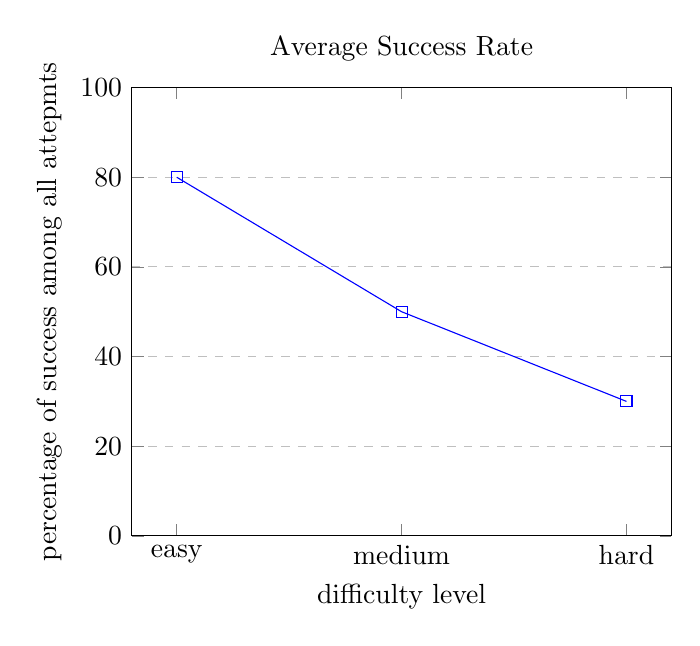
\begin{tikzpicture}
        \begin{axis}[
            title={Average Success Rate},
            xlabel={difficulty level},
            ylabel={percentage of success among all attepmts},
            ymin=0, ymax=100,
            xtick=data,
            xticklabels={easy, medium, hard,},
            ytick={0,20,40,60,80,100},
            legend pos=north west,
            ymajorgrids=true,
            grid style=dashed,
        ]

            \addplot[
                color=blue,
                mark=square,
                ]
                coordinates {
                (1,80)
                (2,50)
                (3,30)
                };
        \end{axis}
    \end{tikzpicture}

    Here are the final matches for the datasets. For each ground dataset, 3 images are provided illustrating the
    matches in easy, medium and hard aerial point clouds. The yellow pixels refer to the aerial point cloud(source)
    and green pixels are related to the ground point cloud(template). The axes of the graph are scaled in meters multiplied
    by a resolution value. This resolution is either 3.3 or 6.6 and is because of variations in the density of points
    and for a more accurate representation of the grid maps.

    For each ground dataset that has at least one successful result, a table of detailed errors of transformation
    in meters, i.e. distance between the center of source and template images, scale in percentage, and angle in
    degrees is provided.

    % 4_3_3
    \newpage
    \begin{figure}[p]
        \centering
        \begin{subfigure}{0.45\textwidth}
            \centering
            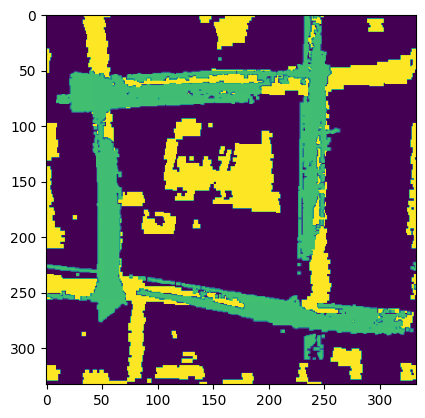
\includegraphics[width=\linewidth]{images/full/easy/4_3_3_easy}
            \caption{Easy: \textcolor{teal}{Success}}
            \label{fig:4_3_3_easy}
        \end{subfigure}
        \hfill
        \begin{subfigure}{0.45\textwidth}
            \centering
            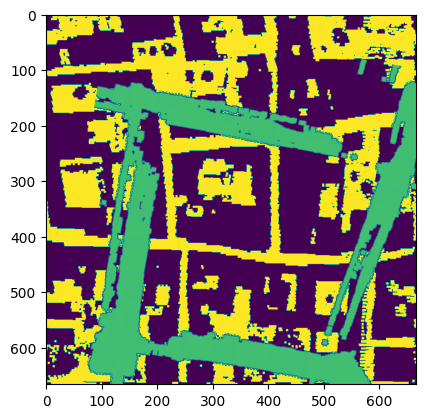
\includegraphics[width=\linewidth]{images/full/medium/4_3_3_medium}
            \caption{Medium: \textcolor{red}{Failed}}
            \label{fig:4_3_3_medium}
        \end{subfigure}

        \vspace{1em}

        \begin{subfigure}{0.45\textwidth}
            \centering
            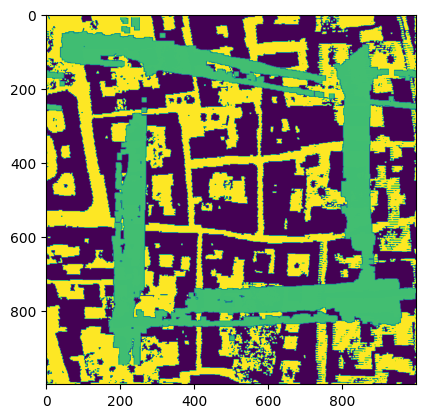
\includegraphics[width=\linewidth]{images/full/hard/4_3_3_hard}
            \caption{Hard: \textcolor{red}{Failed}}
            \label{fig:4_3_3_hard}
        \end{subfigure}
        \hfill

        \caption{Dataset 1}
        \label{fig:res_4_3_3}
    \end{figure}

    \begin{table}[p]
        \centering
        \begin{tabular}{|c|c|c|c|}
          \hline
          \textbf{Errors:} & \textbf{Transformation} & \textbf{Scale} & \textbf{Rotation} \\
          \hline
          \textbf{Easy} & 0.50m & +3.5\% & +2° \\
          \hline
          \textbf{Medium} & - & - & - \\
          \hline
          \textbf{Hard} & - & - & - \\
          \hline
        \end{tabular}
        \caption{Detailed errors of Dataset 1}
        \label{tab:simpletable}
    \end{table}

    % 4_1_3
    \newpage
    \begin{figure}[p]
        \centering
        \begin{subfigure}{0.45\textwidth}
            \centering
            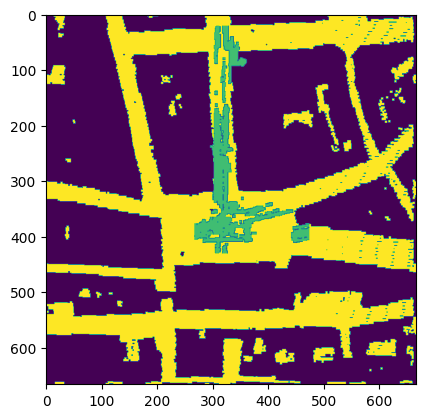
\includegraphics[width=\linewidth]{images/full/easy/4_1_3_easy}
            \caption{Easy: \textcolor{teal}{Success}}
            \label{fig:4_1_3_easy}
        \end{subfigure}
        \hfill
        \begin{subfigure}{0.45\textwidth}
            \centering
            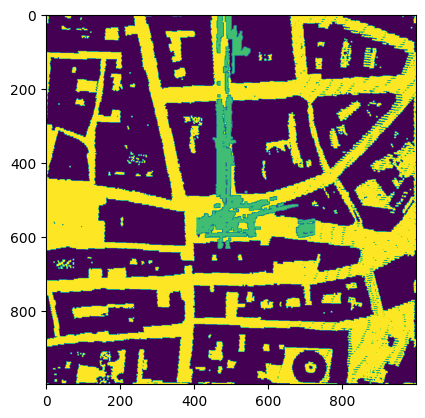
\includegraphics[width=\linewidth]{images/full/medium/4_1_3_medium}
            \caption{Medium: \textcolor{teal}{Success}}
            \label{fig:4_1_3_medium}
        \end{subfigure}

        \vspace{1em}

        \begin{subfigure}{0.45\textwidth}
            \centering
            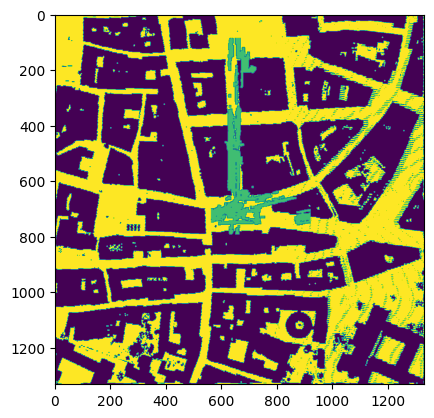
\includegraphics[width=\linewidth]{images/full/hard/4_1_3_hard}
            \caption{Hard: \textcolor{teal}{Success}}
            \label{fig:4_1_3_hard}
        \end{subfigure}
        \hfill

        \caption{Dataset 2}
        \label{fig:res_4_1_3}
    \end{figure}

    \begin{table}[p]
        \centering
        \begin{tabular}{|c|c|c|c|}
          \hline
          \textbf{Errors:} & \textbf{Transformation} & \textbf{Scale} & \textbf{Rotation} \\
          \hline
          \textbf{Easy}   & 3.16m & -8.7\%  & -3° \\
          \hline
          \textbf{Medium} & 6.66  & +7.14\% & -3° \\
          \hline
          \textbf{Hard}   & 26.6  & +16.6\% & -3° \\
          \hline
        \end{tabular}
        \caption{Detailed errors of Dataset 2}
        \label{tab:simpletable}
    \end{table}

    % 5_1_2
    \newpage
    \begin{figure}[p]
        \centering
        \begin{subfigure}{0.45\textwidth}
            \centering
            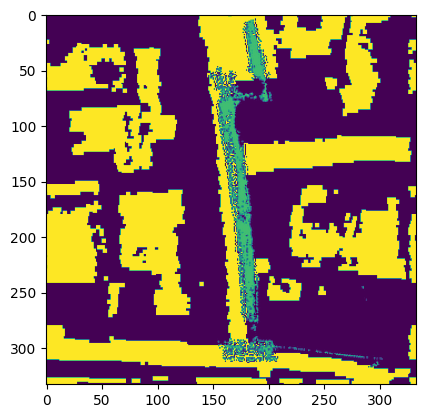
\includegraphics[width=\linewidth]{images/full/easy/5_1_2_easy}
            \caption{Easy: \textcolor{teal}{Success}}
            \label{fig:5_1_2_easy}
        \end{subfigure}
        \hfill
        \begin{subfigure}{0.45\textwidth}
            \centering
            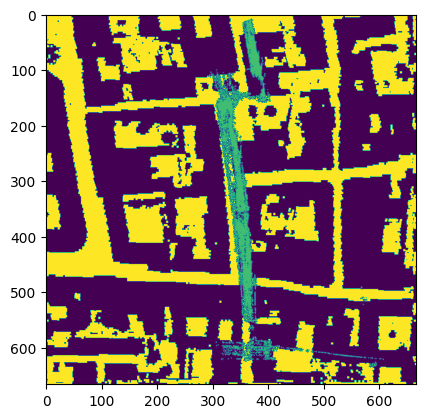
\includegraphics[width=\linewidth]{images/full/medium/5_1_2_medium}
            \caption{Medium: \textcolor{teal}{Success}}
            \label{fig:5_1_2_medium}
        \end{subfigure}

        \vspace{1em}

        \begin{subfigure}{0.45\textwidth}
            \centering
            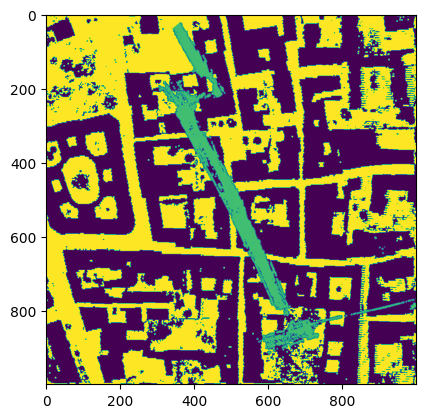
\includegraphics[width=\linewidth]{images/full/hard/5_1_2_hard}
            \caption{Hard: \textcolor{red}{Failed}}
            \label{fig:5_1_2_hard}
        \end{subfigure}
        \hfill

        \caption{Dataset 3}
        \label{fig:res_5_1_2}
    \end{figure}

    \begin{table}[p]
        \centering
        \begin{tabular}{|c|c|c|c|}
          \hline
          \textbf{Errors:} & \textbf{Transformation} & \textbf{Scale} & \textbf{Rotation} \\
          \hline
          \textbf{Easy}   & 1.6m & -4.4\%  & 1° \\
          \hline
          \textbf{Medium} & 4.83m  & +13.3\% & 1° \\
          \hline
          \textbf{Hard}   & -  & - & - \\
          \hline
        \end{tabular}
        \caption{Detailed errors of Dataset 3}
        \label{tab:simpletable}
    \end{table}

    % 4_0_1
    \newpage
    \begin{figure}[p]
        \centering
        \begin{subfigure}{0.45\textwidth}
            \centering
            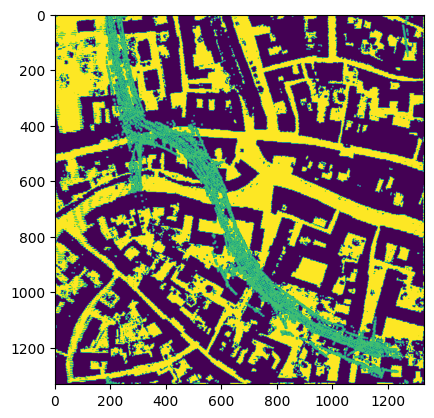
\includegraphics[width=\linewidth]{images/full/easy/4_0_1_easy}
            \caption{Easy: \textcolor{red}{Failed}}
            \label{fig:4_0_1_easy}
        \end{subfigure}
        \hfill
        \begin{subfigure}{0.45\textwidth}
            \centering
            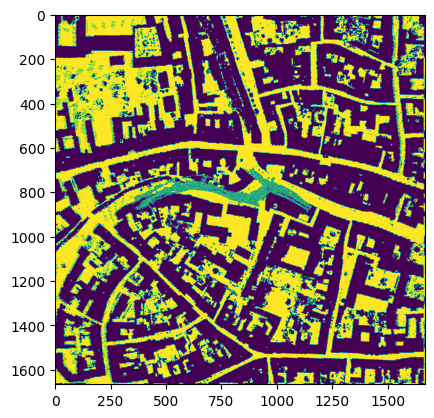
\includegraphics[width=\linewidth]{images/full/medium/4_0_1_medium}
            \caption{Medium: \textcolor{teal}{Success}}
            \label{fig:4_0_1_medium}
        \end{subfigure}

        \vspace{1em}

        \begin{subfigure}{0.45\textwidth}
            \centering
            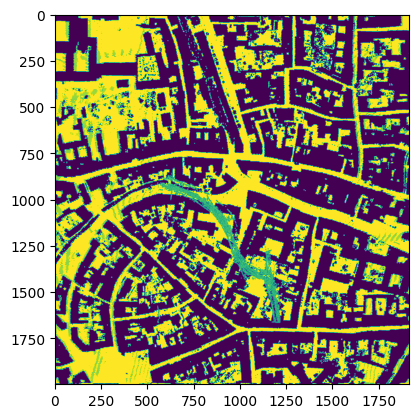
\includegraphics[width=\linewidth]{images/full/hard/4_0_1_hard}
            \caption{Hard: \textcolor{red}{Failed}}
            \label{fig:4_0_1_hard}
        \end{subfigure}
        \hfill

        \caption{Dataset 4}
        \label{fig:res_4_0_1}
    \end{figure}

    \begin{table}[p]
        \centering
        \begin{tabular}{|c|c|c|c|}
          \hline
          \textbf{Errors:} & \textbf{Transformation} & \textbf{Scale} & \textbf{Rotation} \\
          \hline
          \textbf{Easy}   & -  & - & - \\
          \hline
          \textbf{Medium} & 5.62m  & -9.11\% & -3° \\
          \hline
          \textbf{Hard}   & -  & - & - \\
          \hline
        \end{tabular}
        \caption{Detailed errors of Dataset 3}
        \label{tab:simpletable}
    \end{table}

    % 5_6_2
    \newpage
    \begin{figure}[p]
        \centering
        \begin{subfigure}{0.45\textwidth}
            \centering
            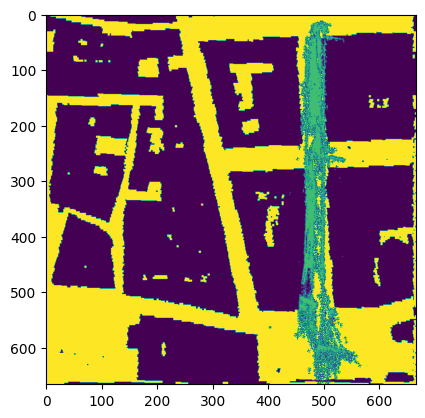
\includegraphics[width=\linewidth]{images/full/easy/5_6_2_easy}
            \caption{Easy: \textcolor{teal}{Success}}
            \label{fig:5_6_2_easy}
        \end{subfigure}
        \hfill
        \begin{subfigure}{0.45\textwidth}
            \centering
            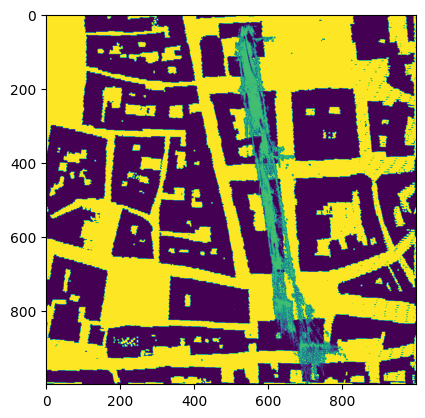
\includegraphics[width=\linewidth]{images/full/medium/5_6_2_medium}
            \caption{Medium: \textcolor{teal}{Success}}
            \label{fig:5_6_2_medium}
        \end{subfigure}

        \vspace{1em}

        \begin{subfigure}{0.45\textwidth}
            \centering
            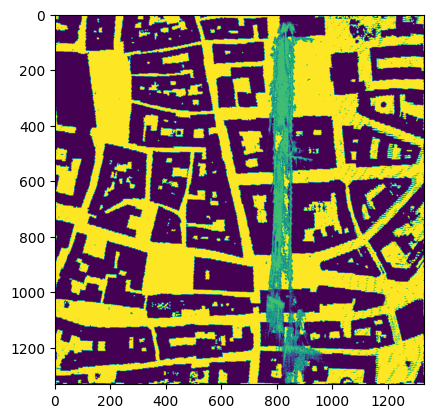
\includegraphics[width=\linewidth]{images/full/hard/5_6_2_hard}
            \caption{Hard: \textcolor{teal}{Success}}
            \label{fig:5_6_2_hard}
        \end{subfigure}
        \hfill

        \caption{Dataset 5}
        \label{fig:res_5_6_2}
    \end{figure}

    \begin{table}[p]
        \centering
        \begin{tabular}{|c|c|c|c|}
          \hline
          \textbf{Errors:} & \textbf{Transformation} & \textbf{Scale} & \textbf{Rotation} \\
          \hline
          \textbf{Easy}   & <1m  & -9.1\% & -3° \\
          \hline
          \textbf{Medium} & #TODO  & +27.2\% & +7° \\
          \hline
          \textbf{Hard}   & #TODO  & +81.2\% & -3° \\
          \hline
        \end{tabular}
        \caption{Detailed errors of Dataset 5}
        \label{tab:simpletable}
    \end{table}

    % 5_7_1
    \newpage
    \begin{figure}[p]
        \centering
        \begin{subfigure}{0.45\textwidth}
            \centering
            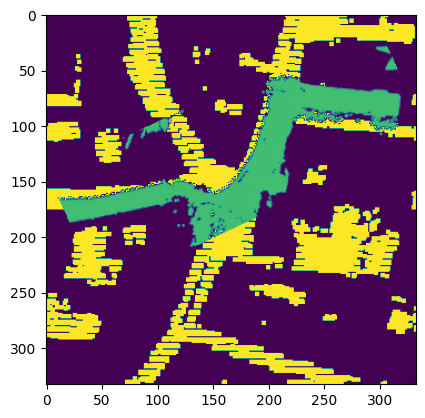
\includegraphics[width=\linewidth]{images/full/easy/5_7_1_easy}
            \caption{Easy: \textcolor{teal}{Success}}
            \label{fig:5_7_1_easy}
        \end{subfigure}
        \hfill
        \begin{subfigure}{0.45\textwidth}
            \centering
            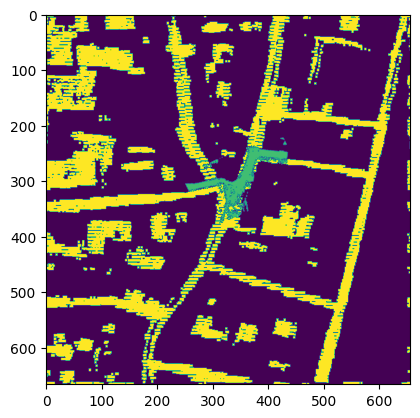
\includegraphics[width=\linewidth]{images/full/medium/5_7_1_medium}
            \caption{Medium: \textcolor{teal}{Success}}
            \label{fig:5_7_1_medium}
        \end{subfigure}

        \vspace{1em}

        \begin{subfigure}{0.45\textwidth}
            \centering
            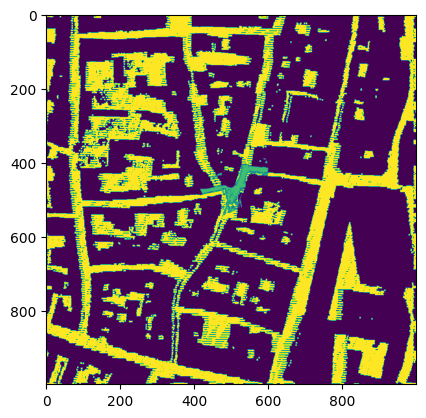
\includegraphics[width=\linewidth]{images/full/hard/5_7_1_hard}
            \caption{Hard: \textcolor{teal}{Success}}
            \label{fig:5_7_1_hard}
        \end{subfigure}
        \hfill

        \caption{Dataset 6}
        \label{fig:res_5_7_1}
    \end{figure}

    \begin{table}[p]
        \centering
        \begin{tabular}{|c|c|c|c|}
          \hline
          \textbf{Errors:} & \textbf{Transformation} & \textbf{Scale} & \textbf{Rotation} \\
          \hline
          \textbf{Easy}   & 1.4m  & +6.1\% & +3° \\
          \hline
          \textbf{Medium} & 3.6m  & +3.3\% & +3° \\
          \hline
          \textbf{Hard}   & 3.5m  & +3.3\% & +3° \\
          \hline
        \end{tabular}
        \caption{Detailed errors of Dataset 6}
        \label{tab:simpletable}
    \end{table}

    % 5_2_4
    \newpage
    \begin{figure}[p]
        \centering
        \begin{subfigure}{0.45\textwidth}
            \centering
            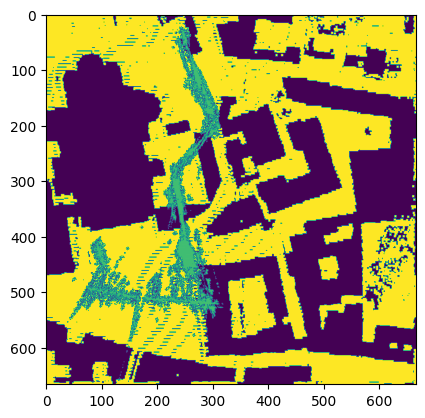
\includegraphics[width=\linewidth]{images/full/easy/5_2_4_easy}
            \caption{Easy: \textcolor{teal}{Success}}
            \label{fig:5_2_4_easy}
        \end{subfigure}
        \hfill
        \begin{subfigure}{0.45\textwidth}
            \centering
            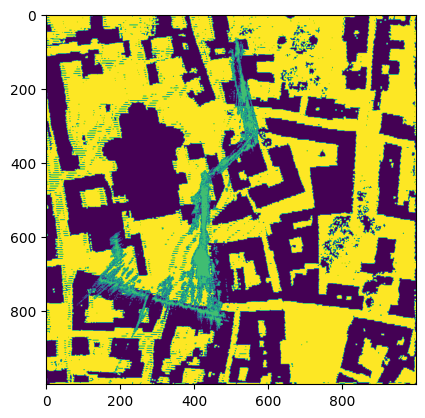
\includegraphics[width=\linewidth]{images/full/medium/5_2_4_medium}
            \caption{Medium: \textcolor{red}{Failed}}
            \label{fig:5_2_4_medium}
        \end{subfigure}

        \vspace{1em}

        \begin{subfigure}{0.45\textwidth}
            \centering
            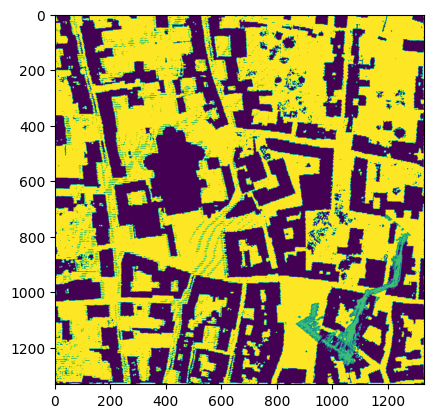
\includegraphics[width=\linewidth]{images/full/hard/5_2_4_hard}
            \caption{Hard: \textcolor{red}{Failed}}
            \label{fig:5_2_4_hard}
        \end{subfigure}
        \hfill

        \caption{Dataset 7}
        \label{fig:res_5_2_4}
    \end{figure}

    \begin{table}[p]
        \centering
        \begin{tabular}{|c|c|c|c|}
          \hline
          \textbf{Errors:} & \textbf{Transformation} & \textbf{Scale} & \textbf{Rotation} \\
          \hline
          \textbf{Easy}   & 34m  & -5.9\% & +4° \\
          \hline
          \textbf{Medium} & -  & - & - \\
          \hline
          \textbf{Hard}   & -  & - & - \\
          \hline
        \end{tabular}
        \caption{Detailed errors of Dataset 7}
        \label{tab:simpletable}
    \end{table}

    % 5_7_2
    \newpage
    \begin{figure}[p]
        \centering
        \begin{subfigure}{0.45\textwidth}
            \centering
            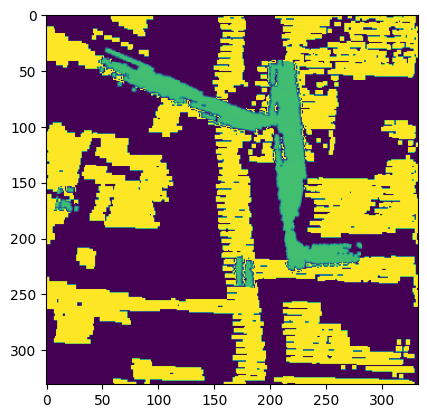
\includegraphics[width=\linewidth]{images/full/easy/5_7_2_easy}
            \caption{Easy: \textcolor{teal}{Success}}
            \label{fig:5_7_2_easy}
        \end{subfigure}
        \hfill
        \begin{subfigure}{0.45\textwidth}
            \centering
            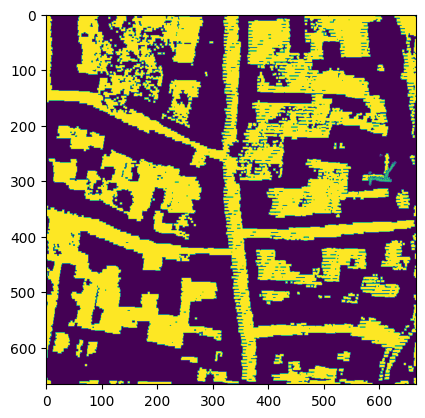
\includegraphics[width=\linewidth]{images/full/medium/5_7_2_medium}
            \caption{Medium: \textcolor{red}{Failed}}
            \label{fig:5_7_2_medium}
        \end{subfigure}

        \vspace{1em}

        \begin{subfigure}{0.45\textwidth}
            \centering
            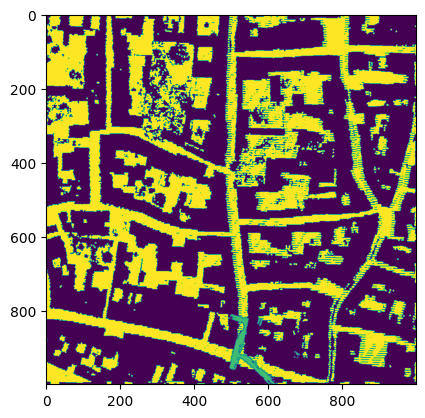
\includegraphics[width=\linewidth]{images/full/hard/5_7_2_hard}
            \caption{Hard: \textcolor{red}{Failed}}
            \label{fig:5_7_2_hard}
        \end{subfigure}
        \hfill

        \caption{Dataset 8}
        \label{fig:res_5_7_2}
    \end{figure}

    \begin{table}[p]
        \centering
        \begin{tabular}{|c|c|c|c|}
          \hline
          \textbf{Errors:} & \textbf{Transformation} & \textbf{Scale} & \textbf{Rotation} \\
          \hline
          \textbf{Easy}   & 17.2m  & -5.2\% & +1° \\
          \hline
          \textbf{Medium} & -  & - & - \\
          \hline
          \textbf{Hard}   & -  & - & - \\
          \hline
        \end{tabular}
        \caption{Detailed errors of Dataset 8}
        \label{tab:simpletable}
    \end{table}

    % 5_6_1
    \newpage
    \begin{figure}[p]
        \centering
        \begin{subfigure}{0.45\textwidth}
            \centering
            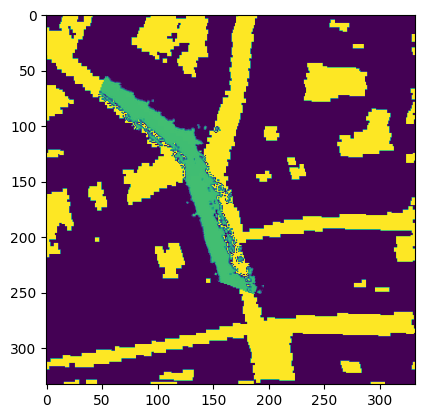
\includegraphics[width=\linewidth]{images/full/easy/5_6_1_easy}
            \caption{Easy: \textcolor{teal}{Success}}
            \label{fig:5_6_1_easy}
        \end{subfigure}
        \hfill
        \begin{subfigure}{0.45\textwidth}
            \centering
            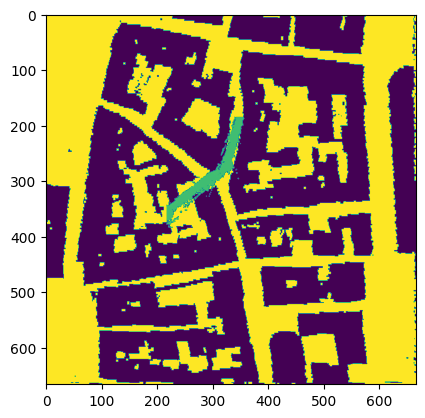
\includegraphics[width=\linewidth]{images/full/medium/5_6_1_medium}
            \caption{Medium: \textcolor{red}{Failed}}
            \label{fig:5_6_1_medium}
        \end{subfigure}

        \vspace{1em}

        \begin{subfigure}{0.45\textwidth}
            \centering
            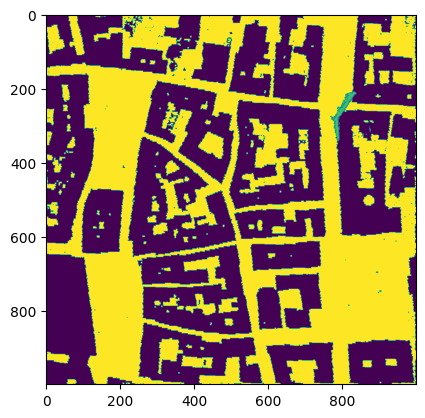
\includegraphics[width=\linewidth]{images/full/hard/5_6_1_hard}
            \caption{Hard: \textcolor{red}{Failed}}
            \label{fig:5_6_1_hard}
        \end{subfigure}
        \hfill

        \caption{Dataset 9}
        \label{fig:res_5_7_2}
    \end{figure}

    \begin{table}[p]
        \centering
        \begin{tabular}{|c|c|c|c|}
          \hline
          \textbf{Errors:} & \textbf{Transformation} & \textbf{Scale} & \textbf{Rotation} \\
          \hline
          \textbf{Easy}   & <1m  & -1.33\% & -3° \\
          \hline
          \textbf{Medium} & -  & - & - \\
          \hline
          \textbf{Hard}   & -  & - & - \\
          \hline
        \end{tabular}
        \caption{Detailed errors of Dataset 9}
        \label{tab:simpletable}
    \end{table}


    % 5_2_3
    \newpage
    \begin{figure}[p]
        \centering
        \begin{subfigure}{0.45\textwidth}
            \centering
            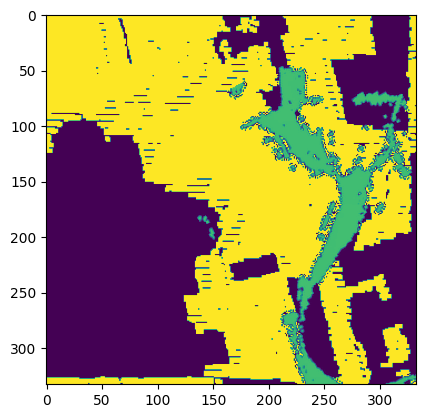
\includegraphics[width=\linewidth]{images/full/easy/5_2_3_easy}
            \caption{Easy: \textcolor{red}{Failed}}
            \label{fig:5_2_3_easy}
        \end{subfigure}
        \hfill
        \begin{subfigure}{0.45\textwidth}
            \centering
            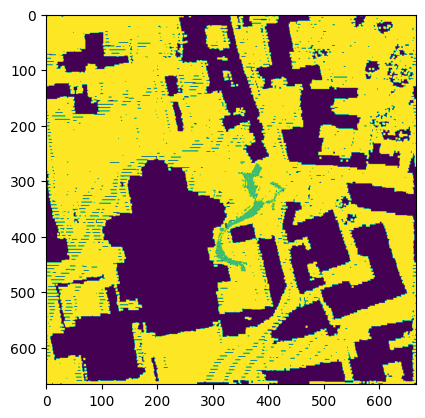
\includegraphics[width=\linewidth]{images/full/medium/5_2_3_medium}
            \caption{Medium: \textcolor{red}{Failed}}
            \label{fig:5_2_4_medium}
        \end{subfigure}

        \vspace{1em}

        \begin{subfigure}{0.45\textwidth}
            \centering
            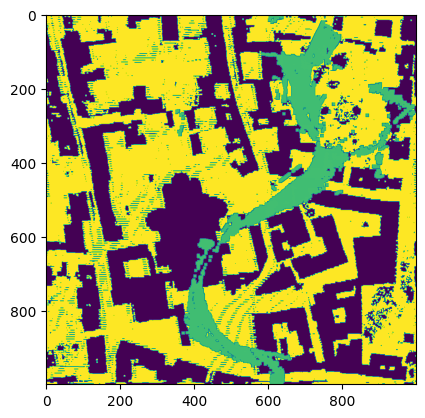
\includegraphics[width=\linewidth]{images/full/hard/5_2_3_hard}
            \caption{Hard: \textcolor{red}{Failed}}
            \label{fig:5_2_3_hard}
        \end{subfigure}
        \hfill

        \caption{Dataset 10}
        \label{fig:res_5_2_3}
    \end{figure}

    \clearpage

    

    \section{Other Approaches}
    \paragraph{Crossroads detection based on handcrafted methods:}
    Correspondence-based registration is a method used in global point cloud registrations. If common features
    could be found, localizing ground point clouds within aerial point clouds would be easier. As it is mentioned
    before, the only common points between those two point clouds are streets which are not distinctive features.
    Instead, crossroads are considered more unique. Therefore, we attempted to detect crossroads in both
    point clouds and directly register them.

    The areas of crossroads are assumed to have more 3D points than the areas of only streets. Because crossroads represent
    the meeting point of two or more streets. Hence, one approach for crossroads detection is selecting points with
    a higher density of neighboring points. However, finding appropriate thresholds for density and the radius to
    select neighboring points were too challenging due to variations in street width, difficulty in distinguishing
    between flat grounds (e.g., yards and gardens) and streets, and differing 3D point densities in ground point
    clouds. We tried to simplify the problem using methods such as uniform point distribution and erosion techniques
    to remove border points while retaining the points related to the center of streets, potentially indicating
    crossroads. However, none of these methods provided accurate and robust results. Figure \ref{fig:ply_erosion} shows the
    result of preprocessing methods and Figure \ref{fig:crossroads_det_1} shows the best results of crossroads detection using
    aforementioned handcrafted methods.

    \begin{figure}
        \centering
        \begin{subfigure}{0.45\textwidth}
            \centering
            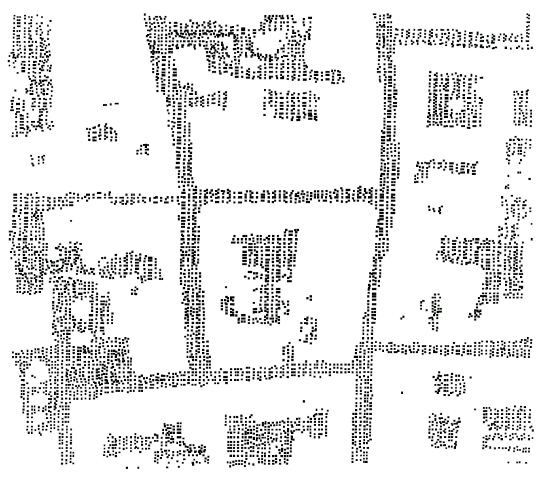
\includegraphics[width=\linewidth]{images/experiment/ply_erosion_0}
        \end{subfigure}
        \hfill
        \begin{subfigure}{0.45\textwidth}
            \centering
            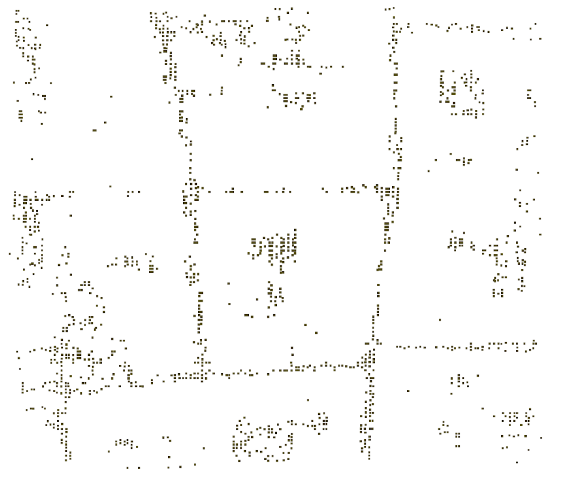
\includegraphics[width=\linewidth]{images/experiment/ply_erosion_1}
        \end{subfigure}
        \caption{Left image: before erosion, Right image: after erosion}
        \label{fig:ply_erosion}
    \end{figure}

    \begin{figure}
    \centering
    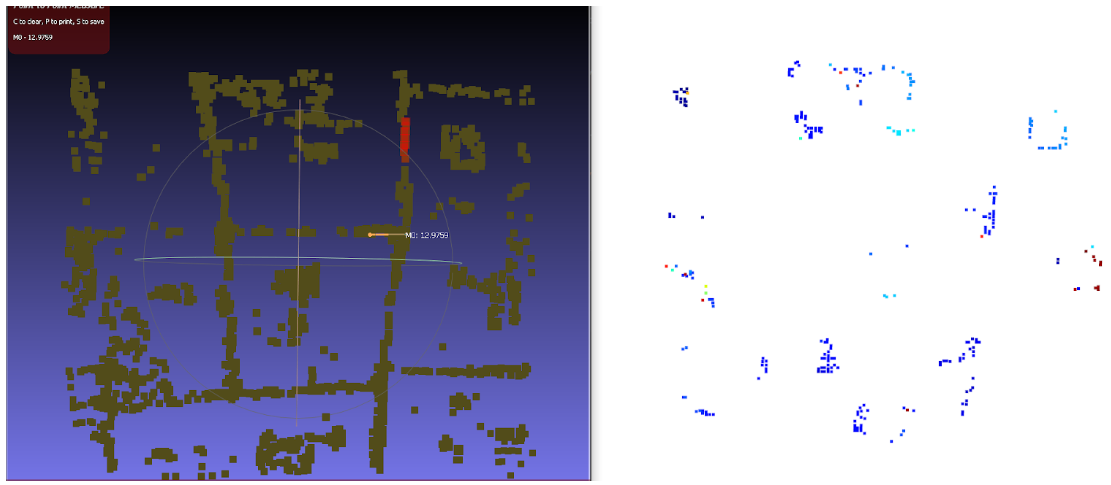
\includegraphics[width=\textwidth,height=\textheight,keepaspectratio]{images/experiment/crossroads_det_1}
    \caption{
        Left image: the actual point cloud,
        Right image: the the same point cloud from the same viewpoint with only crossroads points
    }
    \label{fig:crossroads_det_1}
    \end{figure}

    Another idea involved segmenting the initial ground point cloud, which still contains points from buildings
    and walls, into planes representing the street and multiple building walls. The intersection of at least two building planes
    and the street plane could potentially be identified as crossroads. However, this approach lacked accuracy and
    robustness, particularly in open areas with limited walls, as seen in Dataset 10th. Figure \ref{fig:multi_plane_seg} shows
    the ground point clouds segmented into planes of the street and walls

    \begin{figure}
        \centering
        \begin{subfigure}{0.45\textwidth}
            \centering
            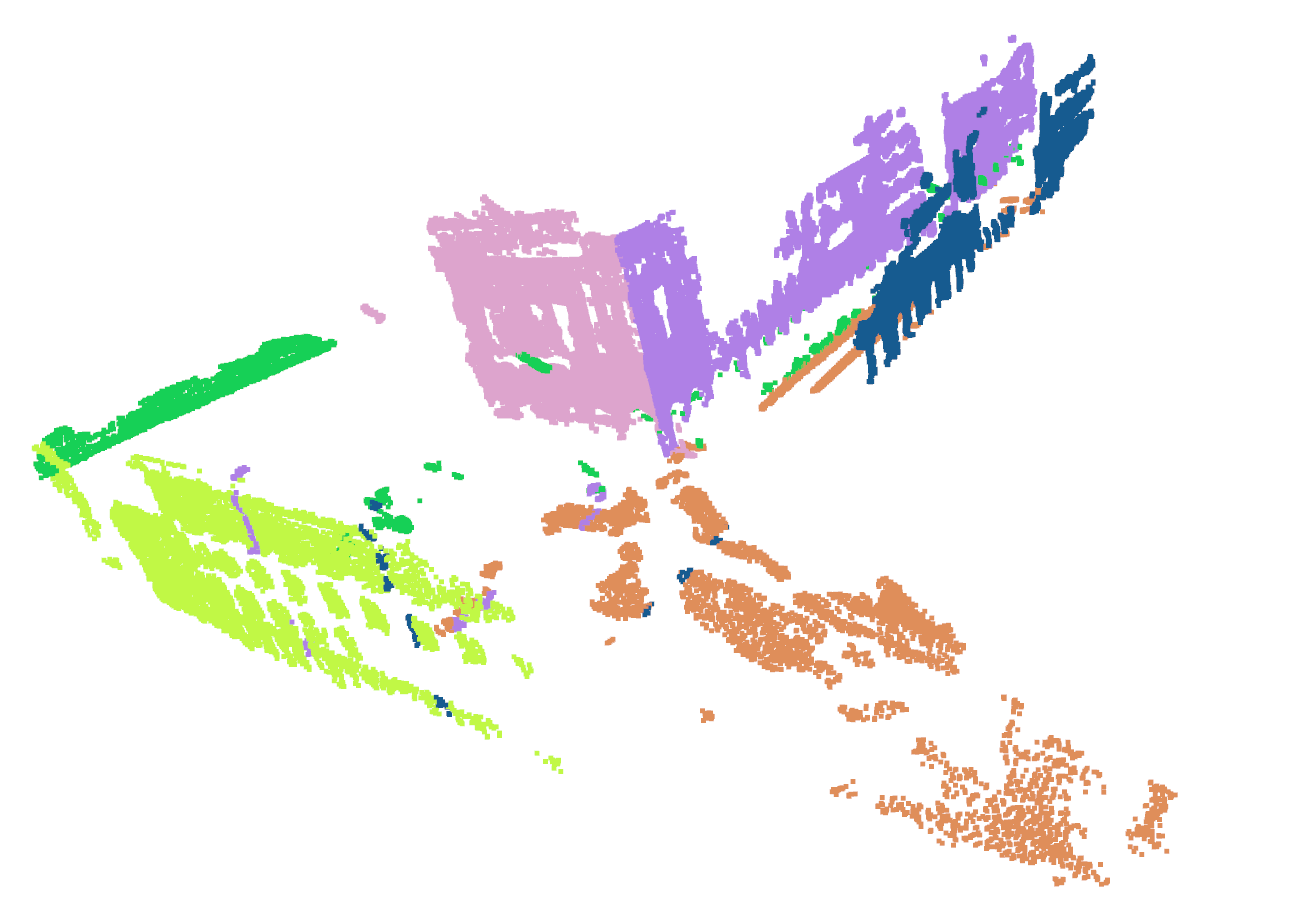
\includegraphics[width=\linewidth]{images/experiment/4_1_3_multi_plane}
        \end{subfigure}
        \hfill
        \begin{subfigure}{0.45\textwidth}
            \centering
            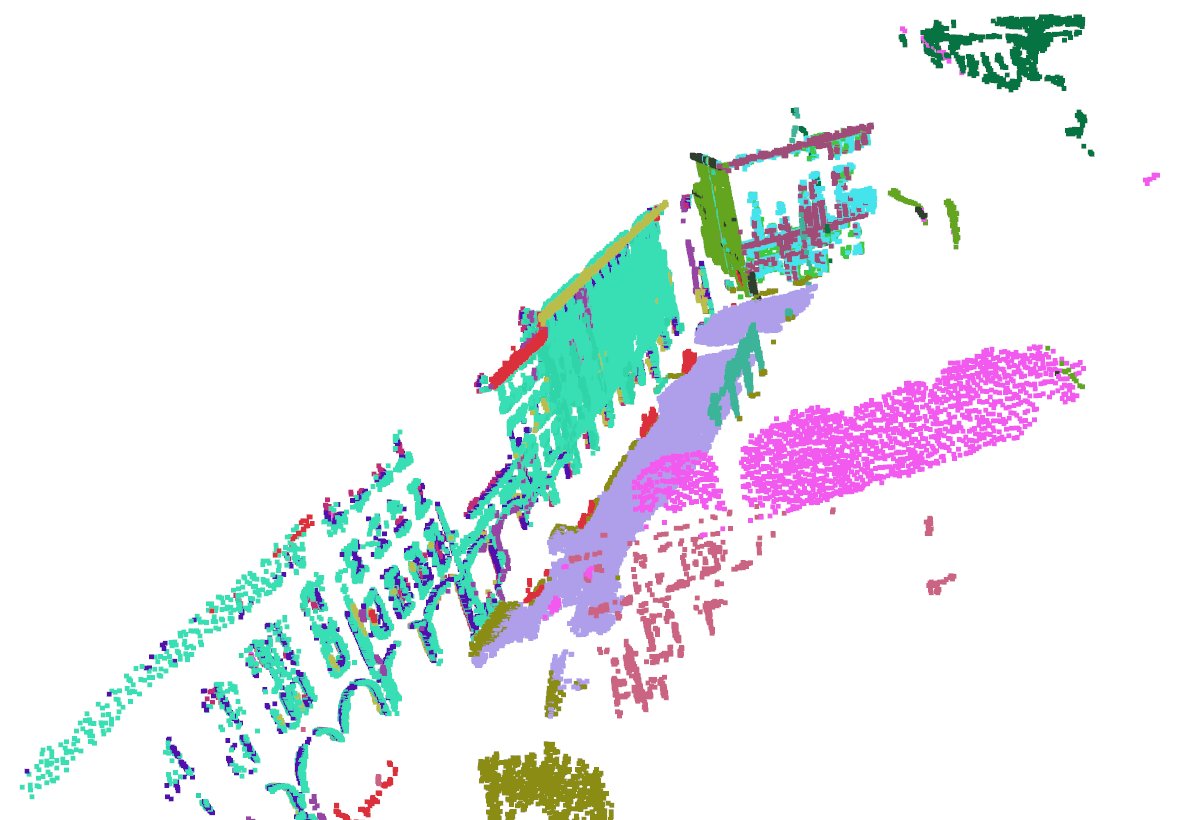
\includegraphics[width=\linewidth]{images/experiment/multi_plane_2}
        \end{subfigure}
        \caption{Ground point clouds segmented into planes of the street and buildings' walls}
        \label{fig:multi_plane_seg}
    \end{figure}

    \clearpage
    \paragraph{Deep Learning based approach:}
    We also explored a Deep Learning approach, utilizing the binary grid maps introduced earlier, as inputs for a
    Convolutional Neural Network to classify them as either crossroads or non-crossroads. Figure \ref{fig:ply_ml_dataset}
    shows a pair of examples of the binary grid maps representing a top-down view of a crossroad and a non-crossroad.
    The model was trained using a small dataset consisting of 10 inputs containing binary grid maps of both classes
    from Dataset 1. Then, we applied the trained model to the entire aerial point cloud of Dataset 1 and filtered out
    points classified as non-crossroads. Figure \ref{fig:multi_plane_seg} illustrates the remaining points identified
    as crossroads which includes points of the 4 main crossroads out of 5. The results demonstrated excellent performance.
    However, to ensure robustness, a significantly larger dataset considering the big 1600m*1000m aerial point cloud
    with approximately 3 million points would be necessary for training.

    \begin{figure}
        \centering
        \begin{subfigure}{0.45\textwidth}
            \centering
            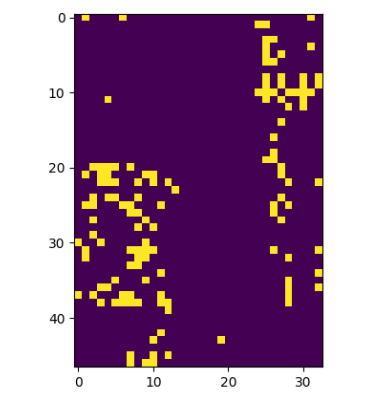
\includegraphics[width=\linewidth]{images/experiment/dataset_0}
            \caption{Random non-crossroads binary grid map}
        \end{subfigure}
        \hfill
        \begin{subfigure}{0.45\textwidth}
            \centering
            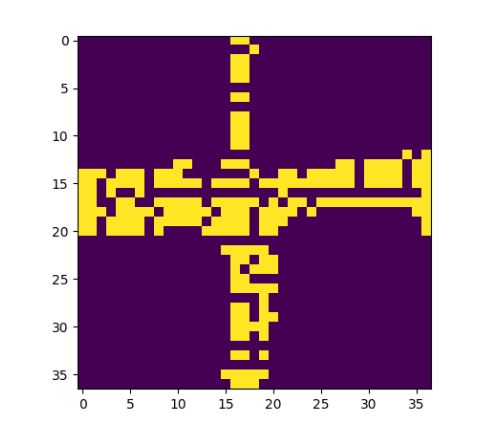
\includegraphics[width=\linewidth]{images/experiment/dataset_1}
            \caption{Random crossroads binary grid map}
        \end{subfigure}
        \caption{Samples of the CNN inputs}
        \label{fig:ply_ml_dataset}
    \end{figure}

    \clearpage
    \section{Reconstruction Details}

    \paragraph{COLMAP} is an open source software, implemented by ~\cite{schoenberger2016sfm} and ~\cite{schoenberger2016mvs},
    that provides 3D reconstruction based on 2D images. Spare and Dense Reconstructions are both implemented in COLMAP.
    Sparse reconstruction results in the 3D point cloud of only the detected features, while dense reconstruction
    refers to the point cloud of all pixels in the input images. Dense reconstruction is achievable after obtaining
    sparse reconstruction with camera poses. By default, It runs PatchMatch algorithm \cite{journals/tog/BarnesSFG09}.
    However, Each step of SfM pipline can be executed separately. Hence, any other algorithm can be replaced by
    its defaults. And, any extra steps, like refinements, can be added to the pipeline.

    \paragraph{Boosting Reconstruction pipeline:}
    The process of Structure from Motion is computationally heavy and not suitable for real-time usage,
    particularly when it comes to dense reconstruction. Table \ref{tab:exe_time} presents the execution time of the sparse reconstruction
    for each step of the SfM algorithm running on our datasets.
    \begin{table}[htb]
        \centering
        \begin{adjustbox}{max width=\textwidth}
            \begin{tabular}{|c|c|c|c|c|c|c|}
                \hline
                 Steps:                 & Max num of features & Feature Extraction & Feature Matching & Bundle Adjustment & total    \\
                \hline
                300 frames(1080p)       & 30000               & 0.85mins           & 1.01mins          & 21.5mins          & 23.36mins \\
                \hline
                300 frames              & 5000                & 0.15mins           & 0.23mins          & 6.74mins          & 7.12mins \\
                \hline
                300 frames(Known poses) & 30000               & 0.73mins           & 1.05mins          & 1.65mins          & 3.43mins \\
                \hline
            \end{tabular}
        \end{adjustbox}
        \caption{The execution time of the sparse reconstruction for each step of the SfM algorithm using Nvidia Rtx3090 graphics}
        \label{tab:exe_time}
    \end{table}

    As can be seen, bundle adjustment is the bottleneck. During our experiments, we noticed that providing an
    initial estimation of camera poses can greatly reduce the number of iterations required for bundle adjustment.
    Hence, we explored the use of existing visual Simultaneous Localization and Mapping (vSLAM) methods to approximate
    the initial camera poses. The best solution we found that using COLMAP sparse reconstruction with low configuration
    parameters, such as lower image resolution and limiting the maximum number of keypoints and matches, just to obtain
    camera poses. Then, COLMAP's sparse reconstruction is re-executing with the initial camera poses and high-quality configuration.
    This trick reduced the execution time significantly such that a dataset of 300 frames was reconstructed in 10 minutes.

    \paragraph{Extra data from GoPro Camera:}
    GoPro cameras come with additional information for the captured videos, such as GPS, IMU.
    https://github.com/gopro/gpmf-parser is the software used to extract these data from video files.
    Here is a sample GPS data of the first 5 seconds:

    \begin{lstlisting}[language=bash,caption={gpmf-parser output},label={lst:lstlisting}]
        VIDEO FRAMERATE:
        59.940 with 31860 frames
        PAYLOAD TIME:
          0.000 to 1.001 seconds
        SCALED DATA:
          GPS5 45.406deg, 11.877deg, 19.839m, 2.418m/s, 2.450m/s,
          GPS5 45.406deg, 11.877deg, 19.831m, 2.432m/s, 2.420m/s,
          GPS5 45.406deg, 11.877deg, 19.816m, 2.489m/s, 2.430m/s,
          GPS5 45.406deg, 11.877deg, 19.811m, 2.501m/s, 2.490m/s,
          GPS5 45.406deg, 11.877deg, 19.807m, 2.501m/s, 2.500m/s,
          GPS5 45.406deg, 11.877deg, 19.821m, 2.495m/s, 2.500m/s,
          GPS5 45.406deg, 11.877deg, 19.828m, 2.503m/s, 2.500m/s,
          GPS5 45.406deg, 11.877deg, 19.830m, 2.505m/s, 2.500m/s,
          GPS5 45.406deg, 11.877deg, 19.825m, 2.520m/s, 2.510m/s,
          GPS5 45.406deg, 11.877deg, 19.819m, 2.493m/s, 2.520m/s,
          GPS5 45.406deg, 11.877deg, 19.822m, 2.472m/s, 2.490m/s,
          GPS5 45.406deg, 11.877deg, 19.820m, 2.471m/s, 2.470m/s,
          GPS5 45.406deg, 11.877deg, 19.822m, 2.494m/s, 2.470m/s,
          GPS5 45.406deg, 11.877deg, 19.790m, 2.448m/s, 2.490m/s,
          GPS5 45.406deg, 11.877deg, 19.775m, 2.444m/s, 2.450m/s,
          GPS5 45.406deg, 11.877deg, 19.775m, 2.434m/s, 2.440m/s,
          GPS5 45.406deg, 11.877deg, 19.759m, 2.404m/s, 2.430m/s,
          GPS5 45.406deg, 11.877deg, 19.763m, 2.412m/s, 2.400m/s,
        PAYLOAD TIME:
          1.001 to 2.002 seconds
        SCALED DATA:
          GPS5 45.406deg, 11.877deg, 19.763m, 2.411m/s, 2.410m/s,
          GPS5 45.406deg, 11.877deg, 19.751m, 2.412m/s, 2.410m/s,
          GPS5 45.406deg, 11.877deg, 19.767m, 2.443m/s, 2.410m/s,
          GPS5 45.406deg, 11.877deg, 19.749m, 2.455m/s, 2.440m/s,
          GPS5 45.406deg, 11.877deg, 19.757m, 2.455m/s, 2.460m/s,
          GPS5 45.406deg, 11.877deg, 19.780m, 2.436m/s, 2.460m/s,
          GPS5 45.406deg, 11.877deg, 19.796m, 2.448m/s, 2.440m/s,
          GPS5 45.406deg, 11.877deg, 19.770m, 2.426m/s, 2.450m/s,
          GPS5 45.406deg, 11.877deg, 19.788m, 2.441m/s, 2.430m/s,
          GPS5 45.406deg, 11.877deg, 19.794m, 2.462m/s, 2.440m/s,
          GPS5 45.406deg, 11.877deg, 19.815m, 2.480m/s, 2.460m/s,
          GPS5 45.406deg, 11.877deg, 19.837m, 2.504m/s, 2.480m/s,
          GPS5 45.406deg, 11.877deg, 19.859m, 2.523m/s, 2.500m/s,
          GPS5 45.406deg, 11.877deg, 19.882m, 2.473m/s, 2.520m/s,
          GPS5 45.406deg, 11.877deg, 19.898m, 2.482m/s, 2.470m/s,
          GPS5 45.406deg, 11.877deg, 19.899m, 2.484m/s, 2.480m/s,
          GPS5 45.406deg, 11.877deg, 19.905m, 2.496m/s, 2.480m/s,
          GPS5 45.406deg, 11.877deg, 19.913m, 2.490m/s, 2.500m/s,
          GPS5 45.406deg, 11.877deg, 19.915m, 2.517m/s, 2.490m/s,
        PAYLOAD TIME:
          2.002 to 3.003 seconds
    \end{lstlisting}

    We saw that initial camera poses can boost SfM pipeline enormously. However, GPS data from GoPro cameras
    are not usable in this process.
    GPS sampling rate is 18 per second. It means there are 18 position data in one second. However, after reviewing
    all GPS data for a long video, we realized that the coordinates are updated every 2 or 3 seconds which is not ideal.
    In SFM, the algorithm finds the coordinates of the camera for each frame. If we want to use GPS data as an initial
    value in SFM, 40 to 60 frames might have the same initial coordinates which doesn't help the algorithm.
    Moreover, GPS data from GPMF metadata has an accuracy of three-tenth of a decimal. We checked this error in
    Google Maps, and the error could be 10 meters. While, SFM has an error of less than a centimeter.

    \paragraph{Calibration and its impact}
    One of the case studies is if giving wider distorted images with manual calibration parameters to the SfM pipeline
    could enhance the accuracy and increase the number of generated point clouds of a wider field of view. We used
    the camera with 2.7k resolution, 60fps, and wide and distorted settings. The camera was calibrated using the
    checkerboard method. Figure \ref{fig:img_distorted} demonstrates an example of undistortion of video frame,
    and Figure \ref{fig:ply_distorted} illustrates the resulting sparse point cloud.
    The generated point cloud has notable error in the street angles, meaning that, from top point of view, the
    streets should be perpendicular to each other. However, Figure \ref{fig:ply_distorted} displays an angle that is less than 90 degrees,
    and the points associated with a ground truth plane are excessively spread out from the generated plane.
    Furthermore, the execution time experienced an exponential increase. For instance, it took approximately
    10 minutes to construct sparse point cloud from the undistorted frames shown in Figure \ref{fig:ply_distorted}
    , whereas the same procedure for the distorted frames required over 2 hours.

    \begin{figure}
        \centering
        \begin{subfigure}{0.45\textwidth}
            \centering
            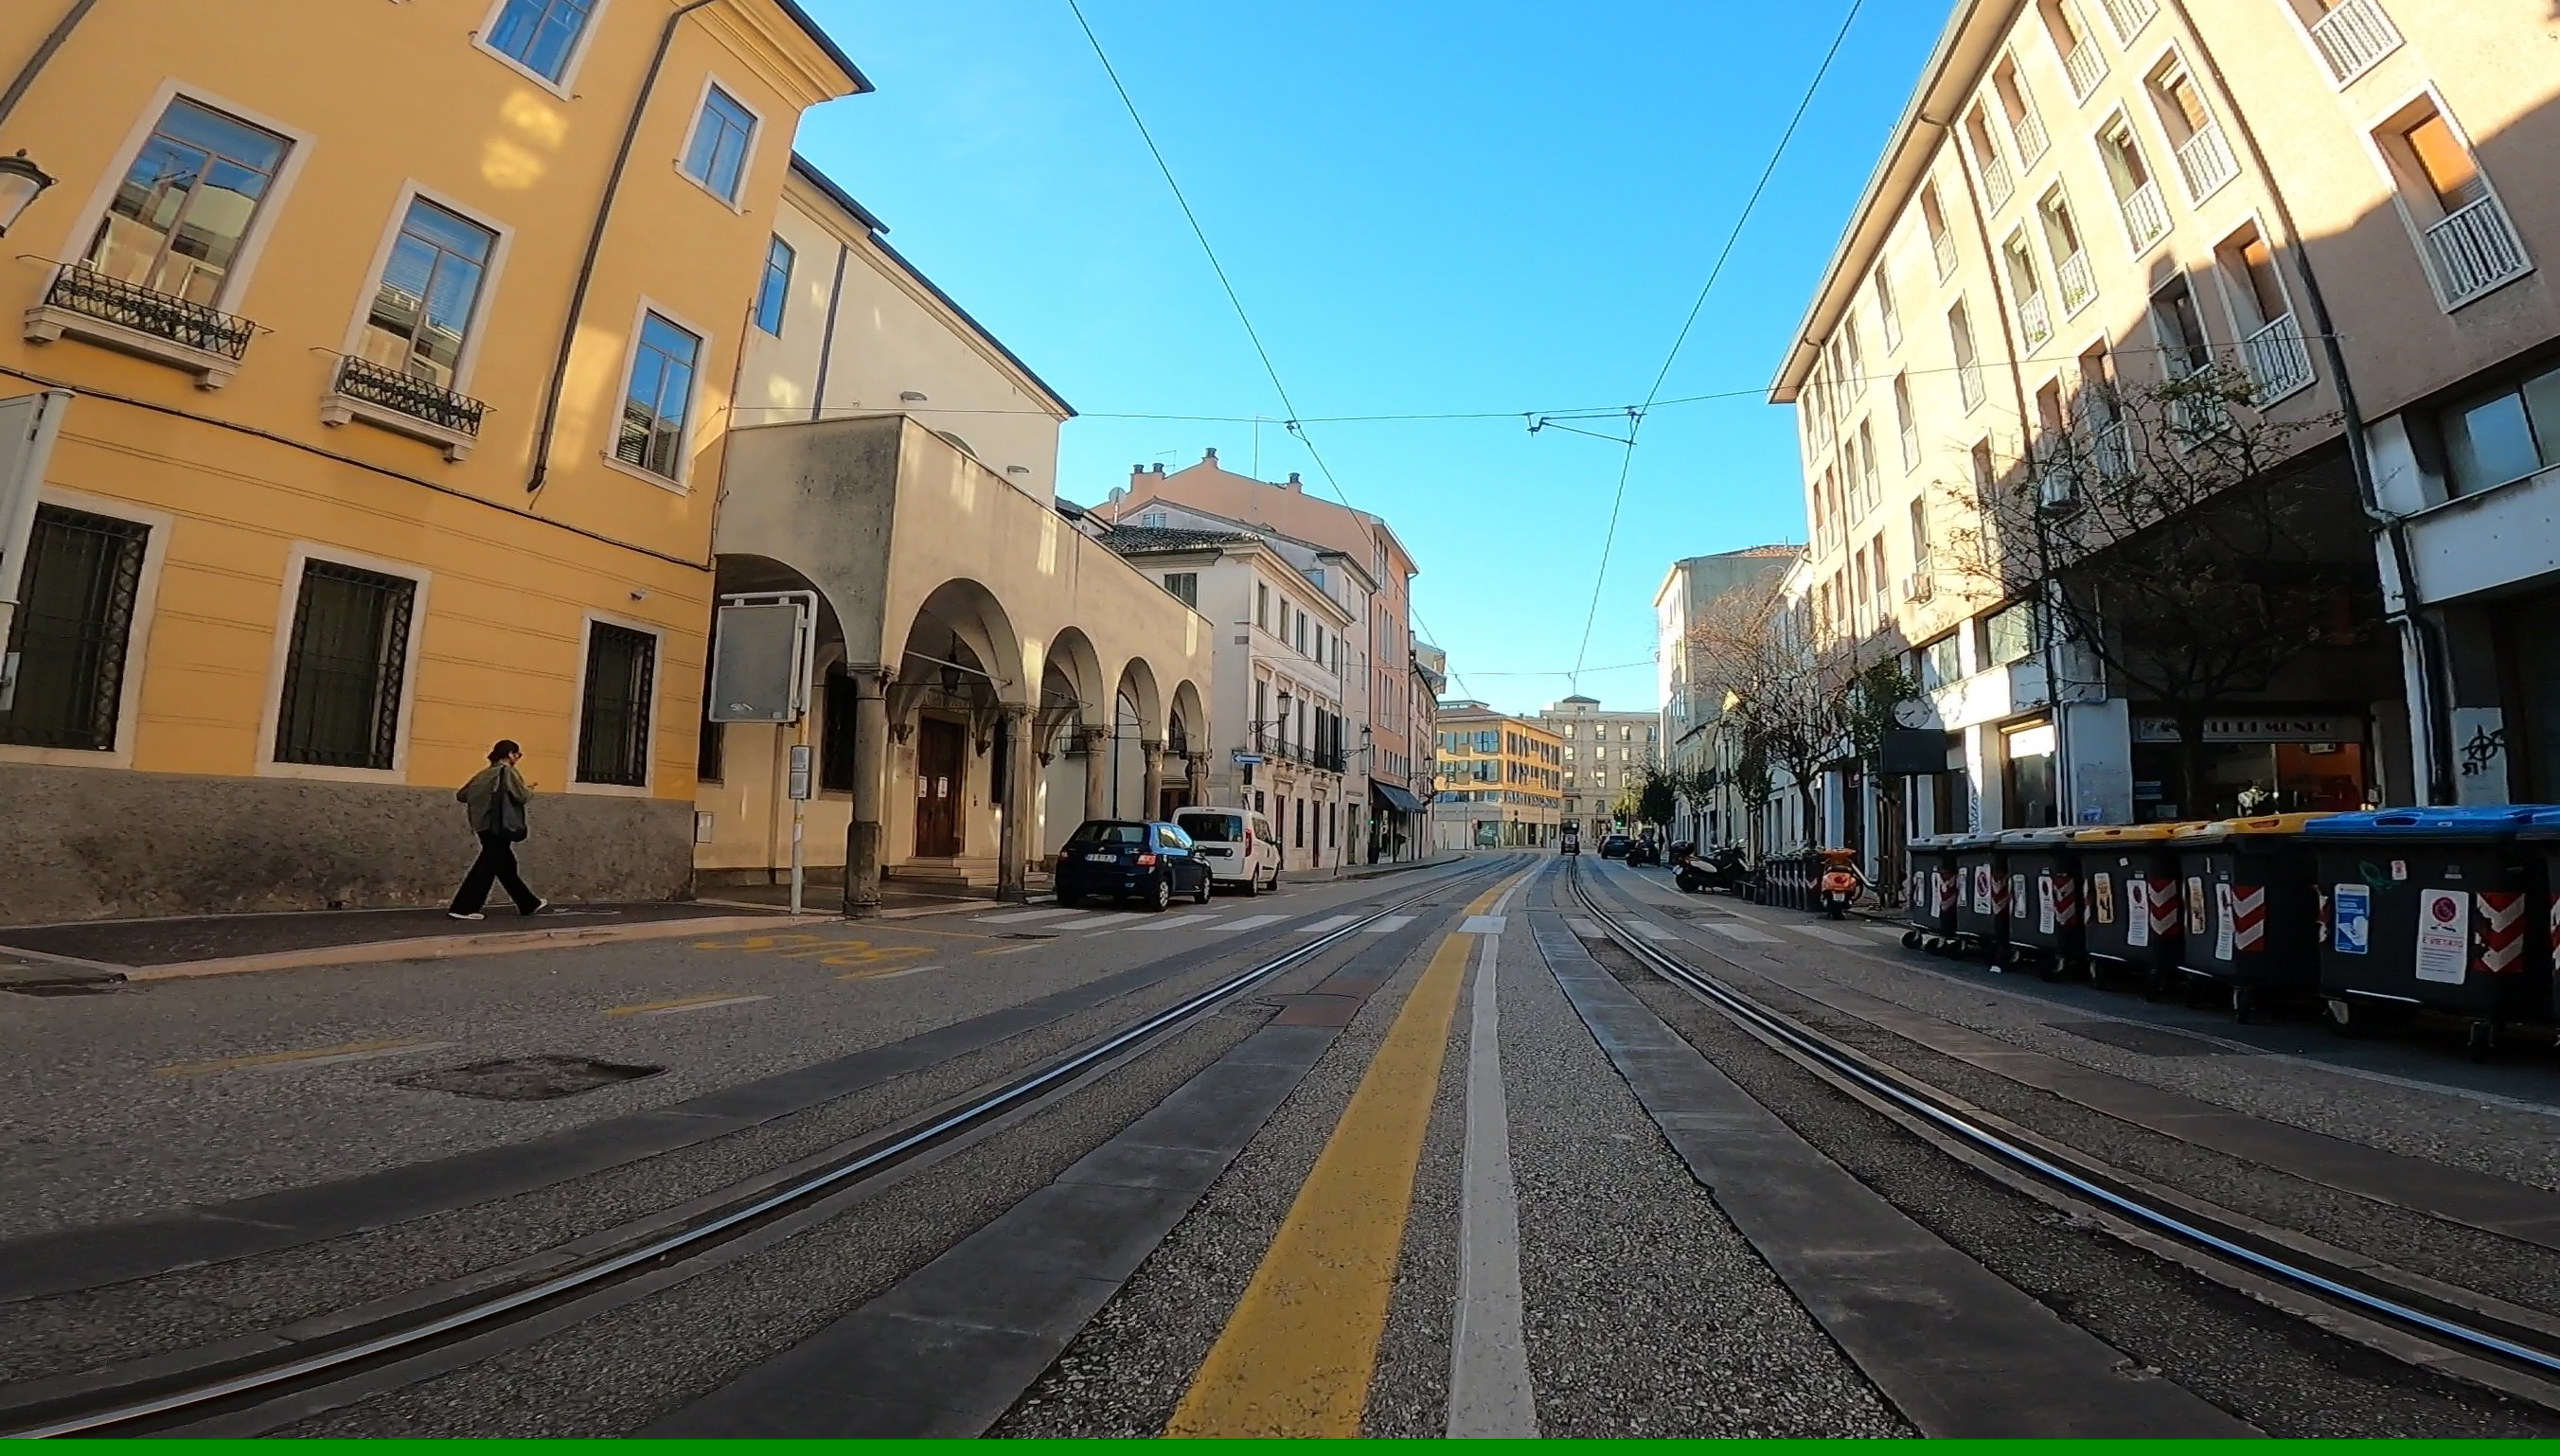
\includegraphics[width=\linewidth]{images/experiment/img_distorted}
            \caption{Distorted frame}
        \end{subfigure}
        \hfill
        \begin{subfigure}{0.45\textwidth}
            \centering
            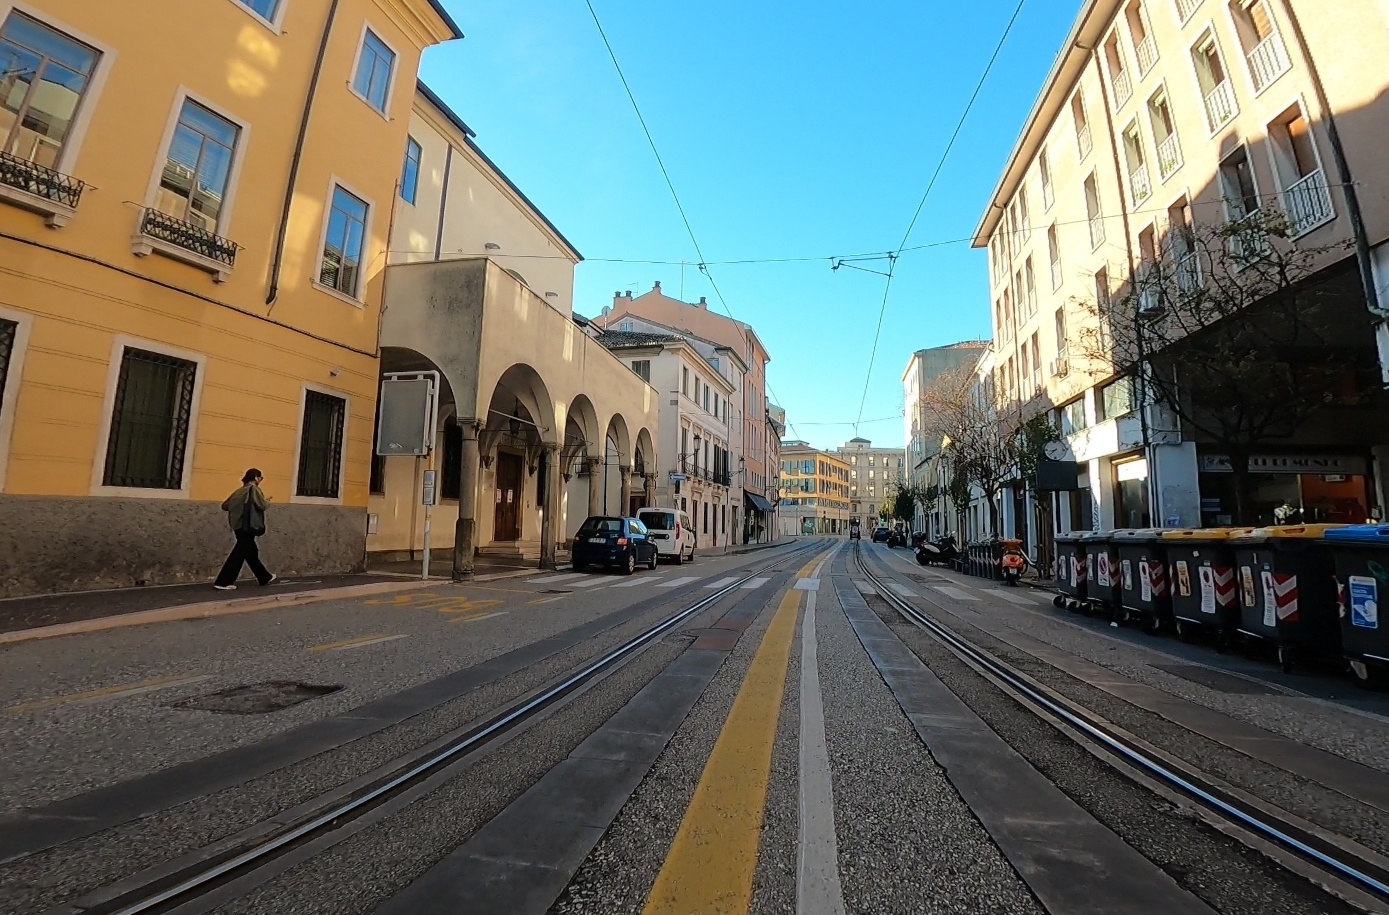
\includegraphics[width=\linewidth]{images/experiment/img_undistorted}
            \caption{Corrected image using calibration parameters}
        \end{subfigure}
        \caption{Samples of distorted and undistorted video frames}
        \label{fig:img_distorted}
    \end{figure}

    \begin{figure}
        \centering
        \begin{subfigure}{0.45\textwidth}
            \centering
            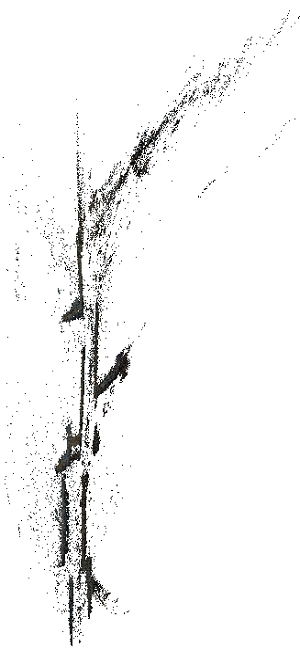
\includegraphics[width=\linewidth]{images/experiment/ply_distorted}
            \caption{From distorted frame}
        \end{subfigure}
        \hfill
        \begin{subfigure}{0.45\textwidth}
            \centering
            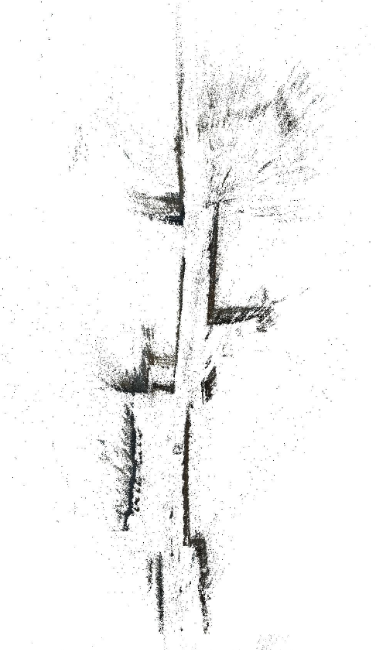
\includegraphics[width=\linewidth]{images/experiment/ply_undistorted}
            \caption{From undistorted frame}
        \end{subfigure}
        \caption{Point clouds generated from distorted and undistorted video frames from top point of view}
        \label{fig:ply_distorted}
    \end{figure}


\end{document}